\documentclass[twoside,single]{lion-msc}

\title{Electrochemical control of single molecules of copper azurin.}
\author{Sebastiaan Van Mulken}
\studentid{0950815}
\supervisor{Biswajit Pradhan \\ \hspace*{\fill}Michel Orrit}
\corrector{Gerard Canters}

\begin{document}
\maketitle



\chapter{Introduction}
With the help of single-molecule fluorescence detection methods, optical studies have made many breakthroughs in the field of physics. Single-molecule fluorescence resonance energy transfer (FRET) is one of the most generally applied techniques. Different kinds of kinetics of proteins, such as redox switching \cite{Akklc}, have been revealed. This switching can be achieved either chemically or electrochemically. Previously, this switching was monitored chemically by adjusting the concentration of oxidizing or reducing agents. In this thesis a new setup is built and tested to achieve switching of proteins electrochemically. Instead of adjusting the concentration of oxidizing or reducing agent a potentiostat will change the potential. This allows more precise and faster changes of potential. With the help of this setup the midpoint potential of blue copper azurin (CuAz) labeled with ATTO 655 (position K122) and other kinetics has been determined. 

This thesis does not only show the results of the new setup, but also gives some insights into how the setup was built. Not only does it describe the steps that did work, but also some of the steps that were not successful. 


\chapter{Theory}
In this chapter we explain the fundamental physics and electrochemistry which are used in the setup.

\section{Fluorescence}
Fluorescence is the property of certain molecules to absorb light at particular wavelengths and emit light at longer wavelengths. These molecules are called fluorophores or fluorescent dyes. A brief interval after absorption - the fluorescence lifetime - the atoms or molecules will emit light of lower energy (longer wavelengths).  Fluorescence is a process governed by three events. All these events occur on different timescales separated by several orders of magnitude, and are summarized in Figure \ref{fluor}.
\begin{figure}[ht!]
\centering
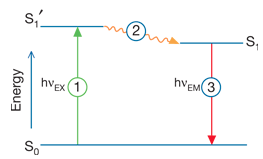
\includegraphics[width=90mm]{fluorescence.jpg}
\caption{The three major events in fluorescence: excitation (1), relaxation (2) and emission (3).} 
\label{fluor}
\end{figure}

\subsection{Excitation}
The first event is excitation. For any molecule, several electronic states exist depending on the total electron energy and the symmetry of the electron spin states. Each state is divided in sub-states - a number of vibrational energy levels associated with vibrations of the atomic nuclei. At room temperature, most molecules lack the internal energy to reach any other state than the lowest vibrational level of the ground state. This ground state is usually an electronic singlet in which all electrons are spin-paired (opposite spins). With the help of a laser, photons with energy $E_{photon}=h \nu_{laser}$ are absorbed by the fluorophores. The absorption of energy happens to any of the closely spaced vibrational energy levels of the excited states. Absorption of light occurs in a few femtoseconds ($10^{-15}s$). It will only occur for specific wavelengths known as the absorption bands. If a photon contains more energy than necessary for an electronic transition, the excess energy is converted into vibrational energy via non-radiative processes. If the energy of a photon is too low, no transition occurs. Excitation of a molecule by absorption normally happens without a change in electron spin-pairing. Therefore, the excited state is also a singlet. Usually the fluorophores are excited to higher vibrational levels of the first or second singlet electronic energy state. Certain transitions have higher probability than others and combined they form an absorption spectrum of the molecule.

\subsection{Vibrational relaxation}
After absorption, several processes occur with varying probabilities. The most likely is relaxation to the lowest vibrational energy level of the first excited state, a process known as internal conversion or vibrational relaxation. This is a loss of energy in a non-radiative matter and has a timescale of a picosecond ($10^{-12}s$) or less. Since a significant number of vibration cycles happen during the excited lifetimes, molecules undergo complete vibrational relaxation. The excess vibrational energy is converted into heat, which is transferred to the neighboring solvent molecules.

\subsection{Emission}
The excited molecule exists in the lowest excited singlet state for a period in the order of nanoseconds ($10^{-9}s$) before relaxing to the ground state. During this relaxation, a photon can be emitted. Because the ground state consists of closely spaced vibrational energy levels, the resulting emission intensity is distributed over a band of wavelengths rather than a sharp line. Most fluorophores can repeat the excitation and emission cycle a lot of times. However, the excited state is more reactive with the surrounding which can result in photobleaching: the molecule is permanently unable to fluoresce. 

Other relaxation pathways compete with the fluorescene emission process. The excited state energy can be dissipated as heat, the excited molecule can collide with another molecule to transfer energy (for example quenching) or intersystem crossing to the lowest excited triplet state can occur. The latter will result in emission of a photon through phosphorescence or a transition back to the excited singlet state that yields delayed fluorescence. Molecules which exhibit the triplet state have a high degree of chemical reactivity, one of the covalent bonds in the molecule may be cleaved by reactions with surrounding molecules resulting in the photo bleaching of the fluorophore.

\section{Fluorescence Resonance Energy Transfer}
Fluorescence resonance energy transfer (FRET) permits determination of the position of two molecules within several nanometers distance, similar to the distance where molecular interactions occur. The process of resonance energy transfer can take place when the donor fluorophore in an electronically excited state transfers its excitation energy to a nearby chromophore (the acceptor). If the fluorescence emission spectrum of the donor molecule overlaps the absorption spectrum of the acceptor molecule and the two are within a minimal spatial radius, the donor can transfer its excitation energy in a non-radiative fashion through dipole-dipole intermolecular coupling. Treating an excited fluorophore as an oscillating dipole, it can exchange energy with a second dipole having a similar resonance frequency. If the acceptor itself is a fluorochrome, increased or sensitised fluorescence emission is observed. By exciting the donor and acceptor molecules with light of wavelengths centred near the absorption maximum of the donor, the detected light will be emitted at wavelengths centred near the emission maximum of the acceptor if FRET has taken place. This resonance energy transfer is not sensitive to the surroundings of a fluorophore. The FRET efficiency is given by:
\begin{equation}
E = \frac{1}{1 + (r/R_{0})^{6}}
\end{equation}
where $r$ is the distance between the donor and acceptor molecule and $R_{0}$ is the F\"oster distance - the distance at which the energy transfer efficiency is 50\%. Related to this efficiency is the lifetime ($\tau_{D}^{'}$ in presence of an acceptor and $\tau_{D}^{'}$ with the absence of an acceptor) and the fluorescence intensity ($F_{D}^{'}$ in pressence of an acceptor and $F_{D}$ with the absence of an acceptor) via the formulas
\begin{equation}
E = 1 - \frac{\tau_{D}^{'}}{\tau_{D}}
\end{equation}
and
\begin{equation}
E = 1 - \frac{F_{D}^{'}}{F_{D}}.
\end{equation}


\section{FluRedox principles and labelled azurin}
In contrast to FRET, FluRedox is based on the change of the overlap integral associated with a change in the optical properties of the redox-active centre upon oxidation and reduction. The optical read-out responds exclusively to the redox state of the protein \cite{Akklc}. 

Azurin is a blue copper protein with an active copper site (see Figure \ref{azurin}). The active centre of azurin has strong characteristic features in its optical absorption spectrum which is dependent on the redox state. It may occur in oxidised ($\textup{Cu}^{2+}$) or reduced ($\textup{Cu}^{+}$) form. Oxidised azurin exhibits a strong absorption band around 600 nm (blue). Fluorescent labelling of this protein makes it suitable for single molecule studies. ATTO 655 is a fluorescent dye with an emission band around 680 nm. The emission band of the dye and the absorption band of the azurin overlap (see Figure \ref{absorption}). When azurin is oxidised, FRET between the dye and the centre quenches the dye fluorescence. This quenching is absent when the protein is in reduced state because its 600 nm absorption has vanished \cite{Tabares2014}.

\begin{figure}[ht!]
\centering
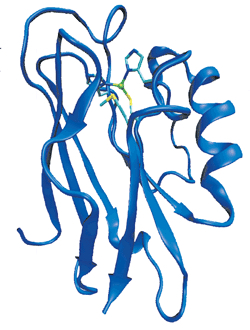
\includegraphics[width=50mm]{azurin1}
\caption{Three dimensional structure of azurin. The green sphere is the copper centre of the protein. Picture is taken from \cite{BORMAN2010}.} 
\label{azurin}
\end{figure}

\begin{figure}[ht!]
\centering
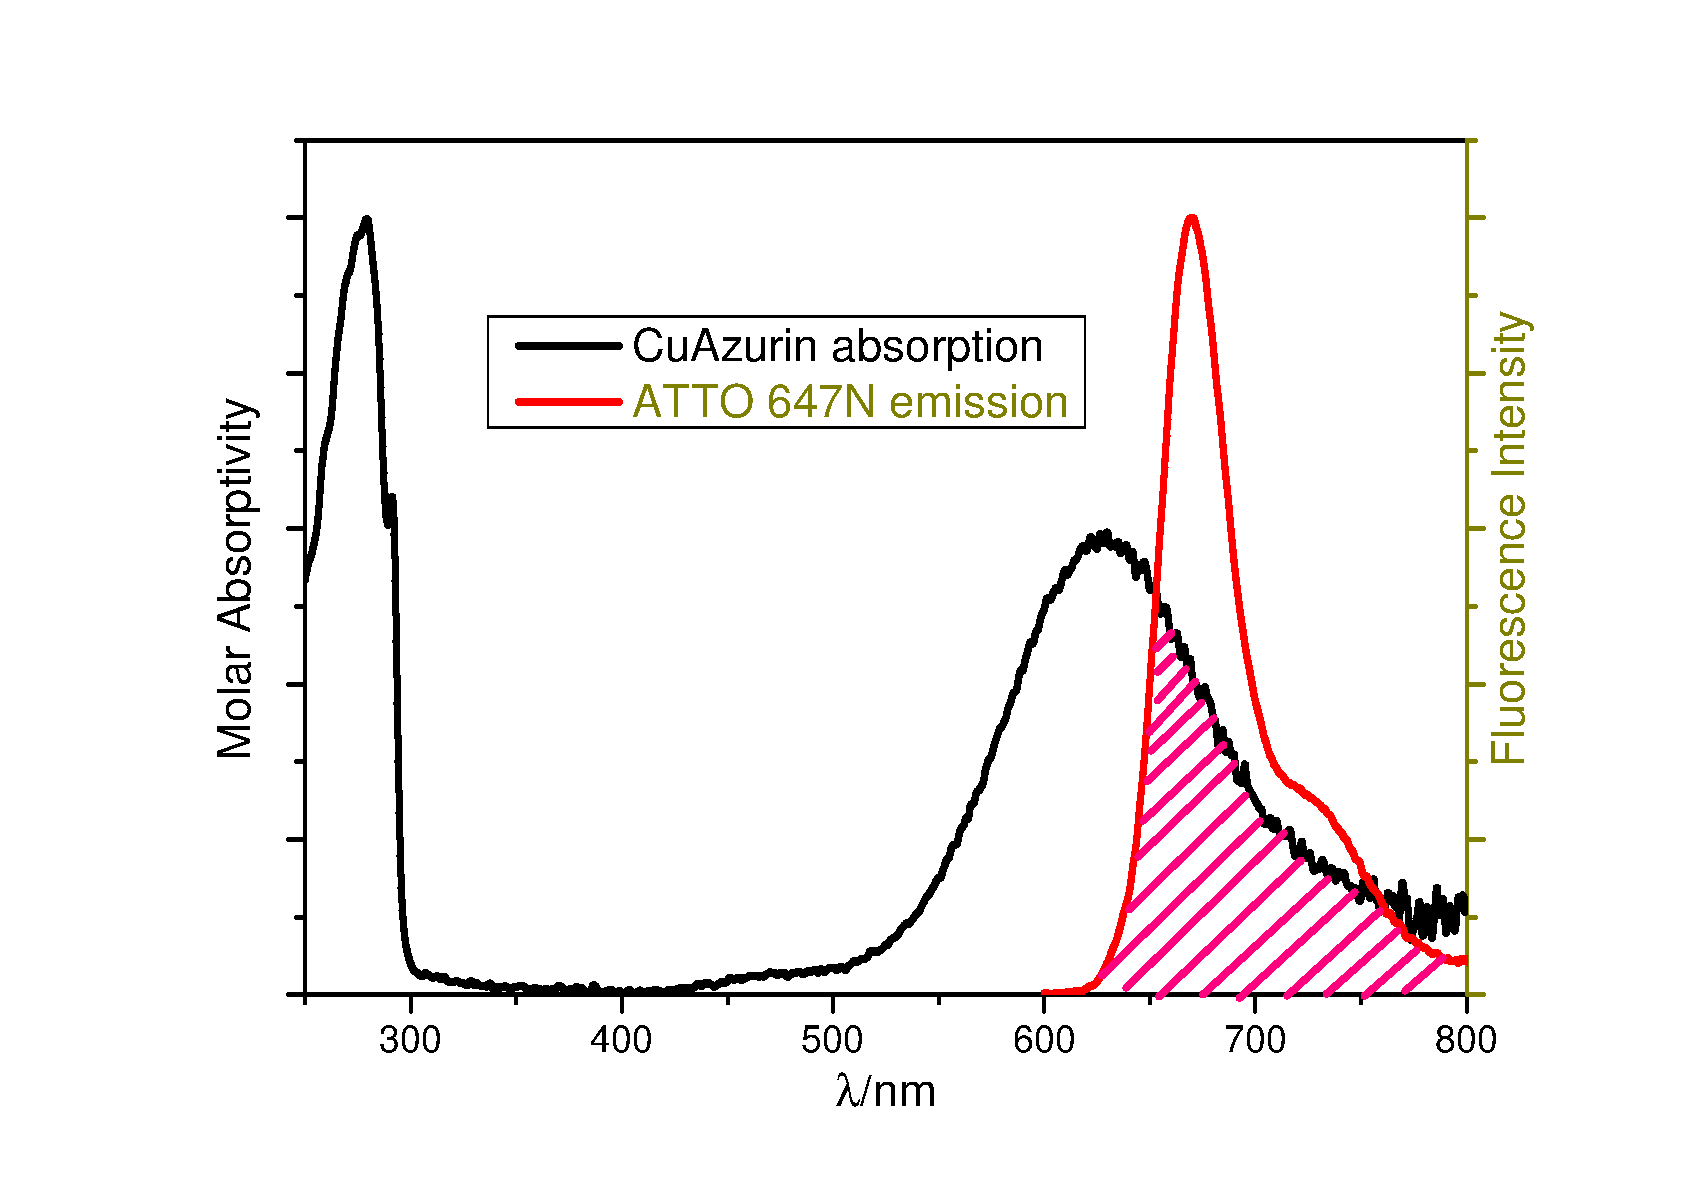
\includegraphics[width=90mm]{absorp.pdf}
\caption{Absorption spectrum of CuAz (black) and the emission spectrum of the fluorescence dye ATTO 655 (red). The overlapping parts are purple marked. The absortion band around 600 nm is absent when azurin is reduced.} 
\label{absorption}
\end{figure}


\section{Single molecules techniques}
It is impossible to open newspapers without stumbling over words that reflect the impact of the life sciences in the modern world. Many speculations and discussions suffer from vagueness since many biological mechanisms are barely known to exist and even less mechanisms are fully understood. New and more precise techniques have made this field grow quickly. With new synthetic fluorophores, the ability to study single proteins at a time is exploited to investigate a variety of dynamics.  One of the ways to get a better understanding of these single proteins is the usage of fluorescence correlation spectroscopy and the usage of confocal microscopes. 

\subsection{Fluorescence Correlation Spectroscopy}
The instrumentation of Fluorescence Correlation Spectroscopy (FCS) is based on an inverted confocal microscope.  A laser beam is directed into a microscope objective via dichroic mirrors and focused on the sample. High numerical apertures are used. Fluorescence light from the sample is collected and passed through the dichroic and emission filters. A pinhole in the image plane blocks the light not originating from the focal region. When concentrations in order of a few - or less - nanomolar of fluorescent particles are applied, single particles can be monitored at a given time. A more detailed description can be found in reference \cite{Schwille}.

The fluorescence intensity collected during the experiments were elaborated using the normalized autocorrelation (AC) function, defined by:
\begin{equation}
G'(\tau) = \frac{\left \langle I(t)I(t + \tau) \right \rangle}{\left \langle I(t)\right \rangle ^{2}}.
\end{equation}
Substracting the normal offset of value 1, this leads to
\begin{equation} \label{AC}
G(\tau) = G'(\tau) - 1 =  \frac{\left \langle \delta I(t)\delta I(t + \tau) \right \rangle}{\left \langle I(t)\right \rangle ^{2}}
\end{equation}
where the brackets  denotes temporal averaging and $\delta I(t) = I(t) - \left \langle I(t)\right \rangle$. The autocorrelation function is the correlation between a signal and the by $\tau$ delayed copy of itself.

\subsection{Confocal Laser Scanning Microscopy}
A Confocal Laser Scanning Microscope (CLSM) is the apparatus we used in this experiment. The CLSM is used to scan a sample. The sample is mounted on a moving piezoelectric scanning stage. This allows sub-micrometer movements. The scanning stage is moved along the confocal volume and the fluorescent signal is collected for each position sampled. Together with the fluorescence intensity, the setup is equipped to record the lifetime of the fluorescence and timetraces with the help of a time-correlated single-photon counting (TCSPC) board. A more detailed description of the setup is found in sections \ref{confo_micro} and \ref{data_coll}.

For this thesis, the Cu-azurin (CuAz) and Zn-azurin (ZnAz) were labeled and immobilized on the sample slide. Surrounded by an electron mediator, different potentials were applied on areas of (10 x 10) $\upmu \textup{m}^{2}$, which have around 30 - 40 immobilized proteins. Initially applying a positive and negative potential, by analysing the fluorescence lifetime and fluorescence intensity, the active CuAz and inactive CuAz/impurities can be identified immediately after taking the images. Since the redox state affects directly the fluorescence lifetime and fluorescence intensity of the dye (see Figure \ref{finding_proteins_1}),  active CuAz is in the dark state when oxidized and in the bright state when reduced. Inactive CuAz/impurities are usually in bright state, independently of the redox state of the surrounding solution. When a single CuAz causes some doubt whether or not it is an active protein, a lifetime graph such as the ones in Figure \ref{lifetime} can be made. CuAz has a typical lifetime of around 2 ns. 
Once we select the active proteins, the signal of the proteins is recorded for different time intervals (usually 30 seconds) resulting in timetraces as shown in Figure \ref{TT_exam}.

\begin{figure}
\begin{subfigure}{.5\textwidth}
  \centering
  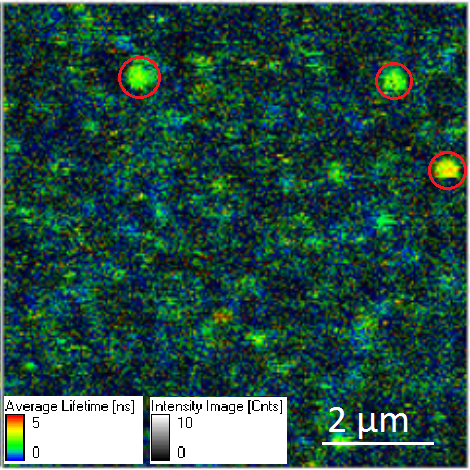
\includegraphics[width=.95 \linewidth]{voorbeeld_protein_2}
  \label{}
\end{subfigure}%
\begin{subfigure}{.5\textwidth}
  \centering
  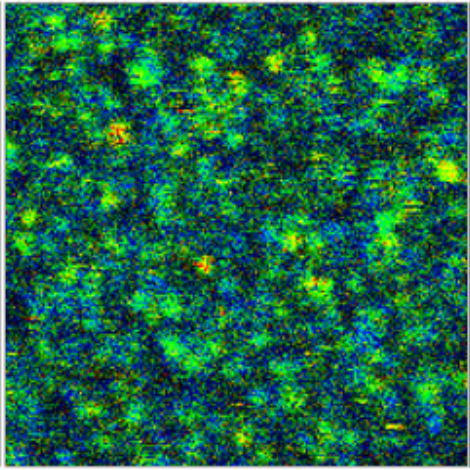
\includegraphics[width=.95 \linewidth]{voorbeeld_protein_1}
  \label{}
\end{subfigure}
\caption{A  (10 x 10) $\upmu \textup{m}^{2}$  lifetime image of an area filled with immobilized Cu-azurin at different potentials. On the right: potential of -100 mV, here the Cu-azurin is reduced (bright state). On the left: potential of +100 mV. The Cu-azurin is oxidised and in the dark state. The bright spots (red circles) in the dark state are either bleached proteins or impurities. A way to get rid of these impurities is by focusing the laser with slightly more power on these spots. Comparing these two pictures immediately shows the active proteins and the non active proteins/impurities.}
\label{finding_proteins_1}
\end{figure}

\begin{figure}[ht!]
\centering
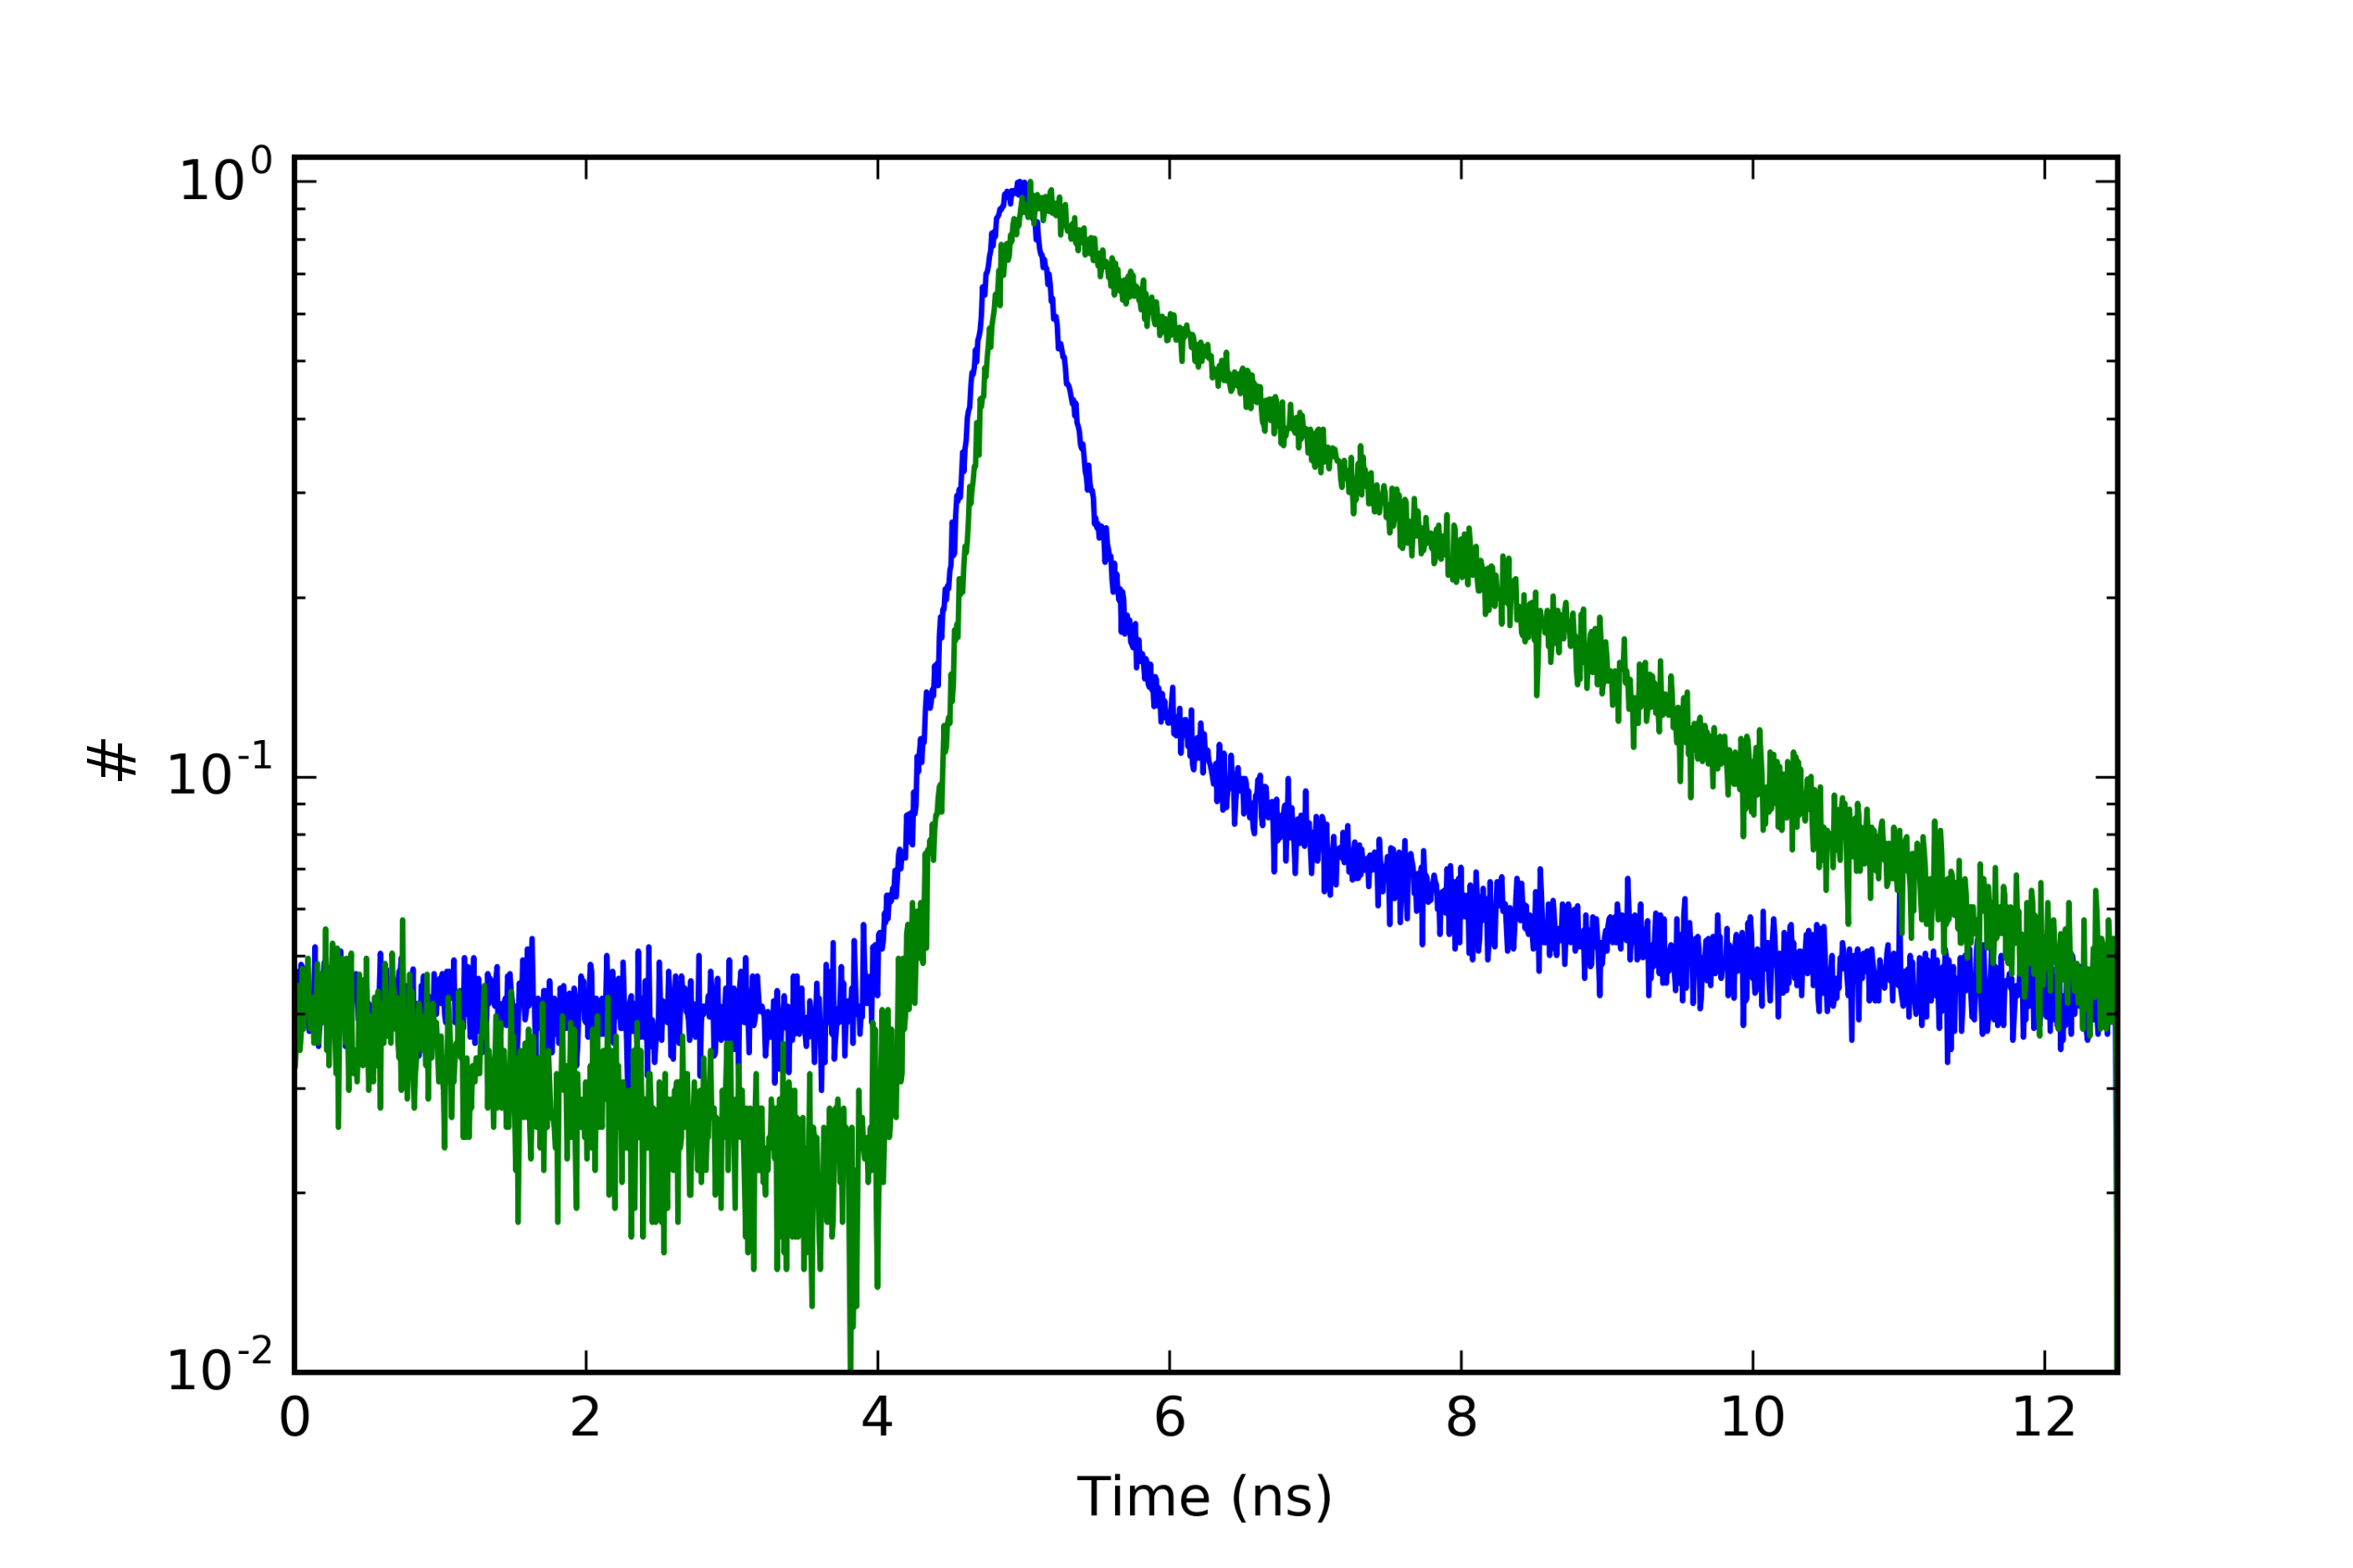
\includegraphics[width= .9 \textwidth]{lifetime.png}
\caption{Lifetime graphs of reduced (green line) and oxidized (blue line) CuAz. Reduced CuAz has a typical lifetime of 2 ns, while it has a lifetime of around 1.6 ns when oxidized.} 
\label{lifetime}
\end{figure}



\begin{figure}[ht!]
\centering
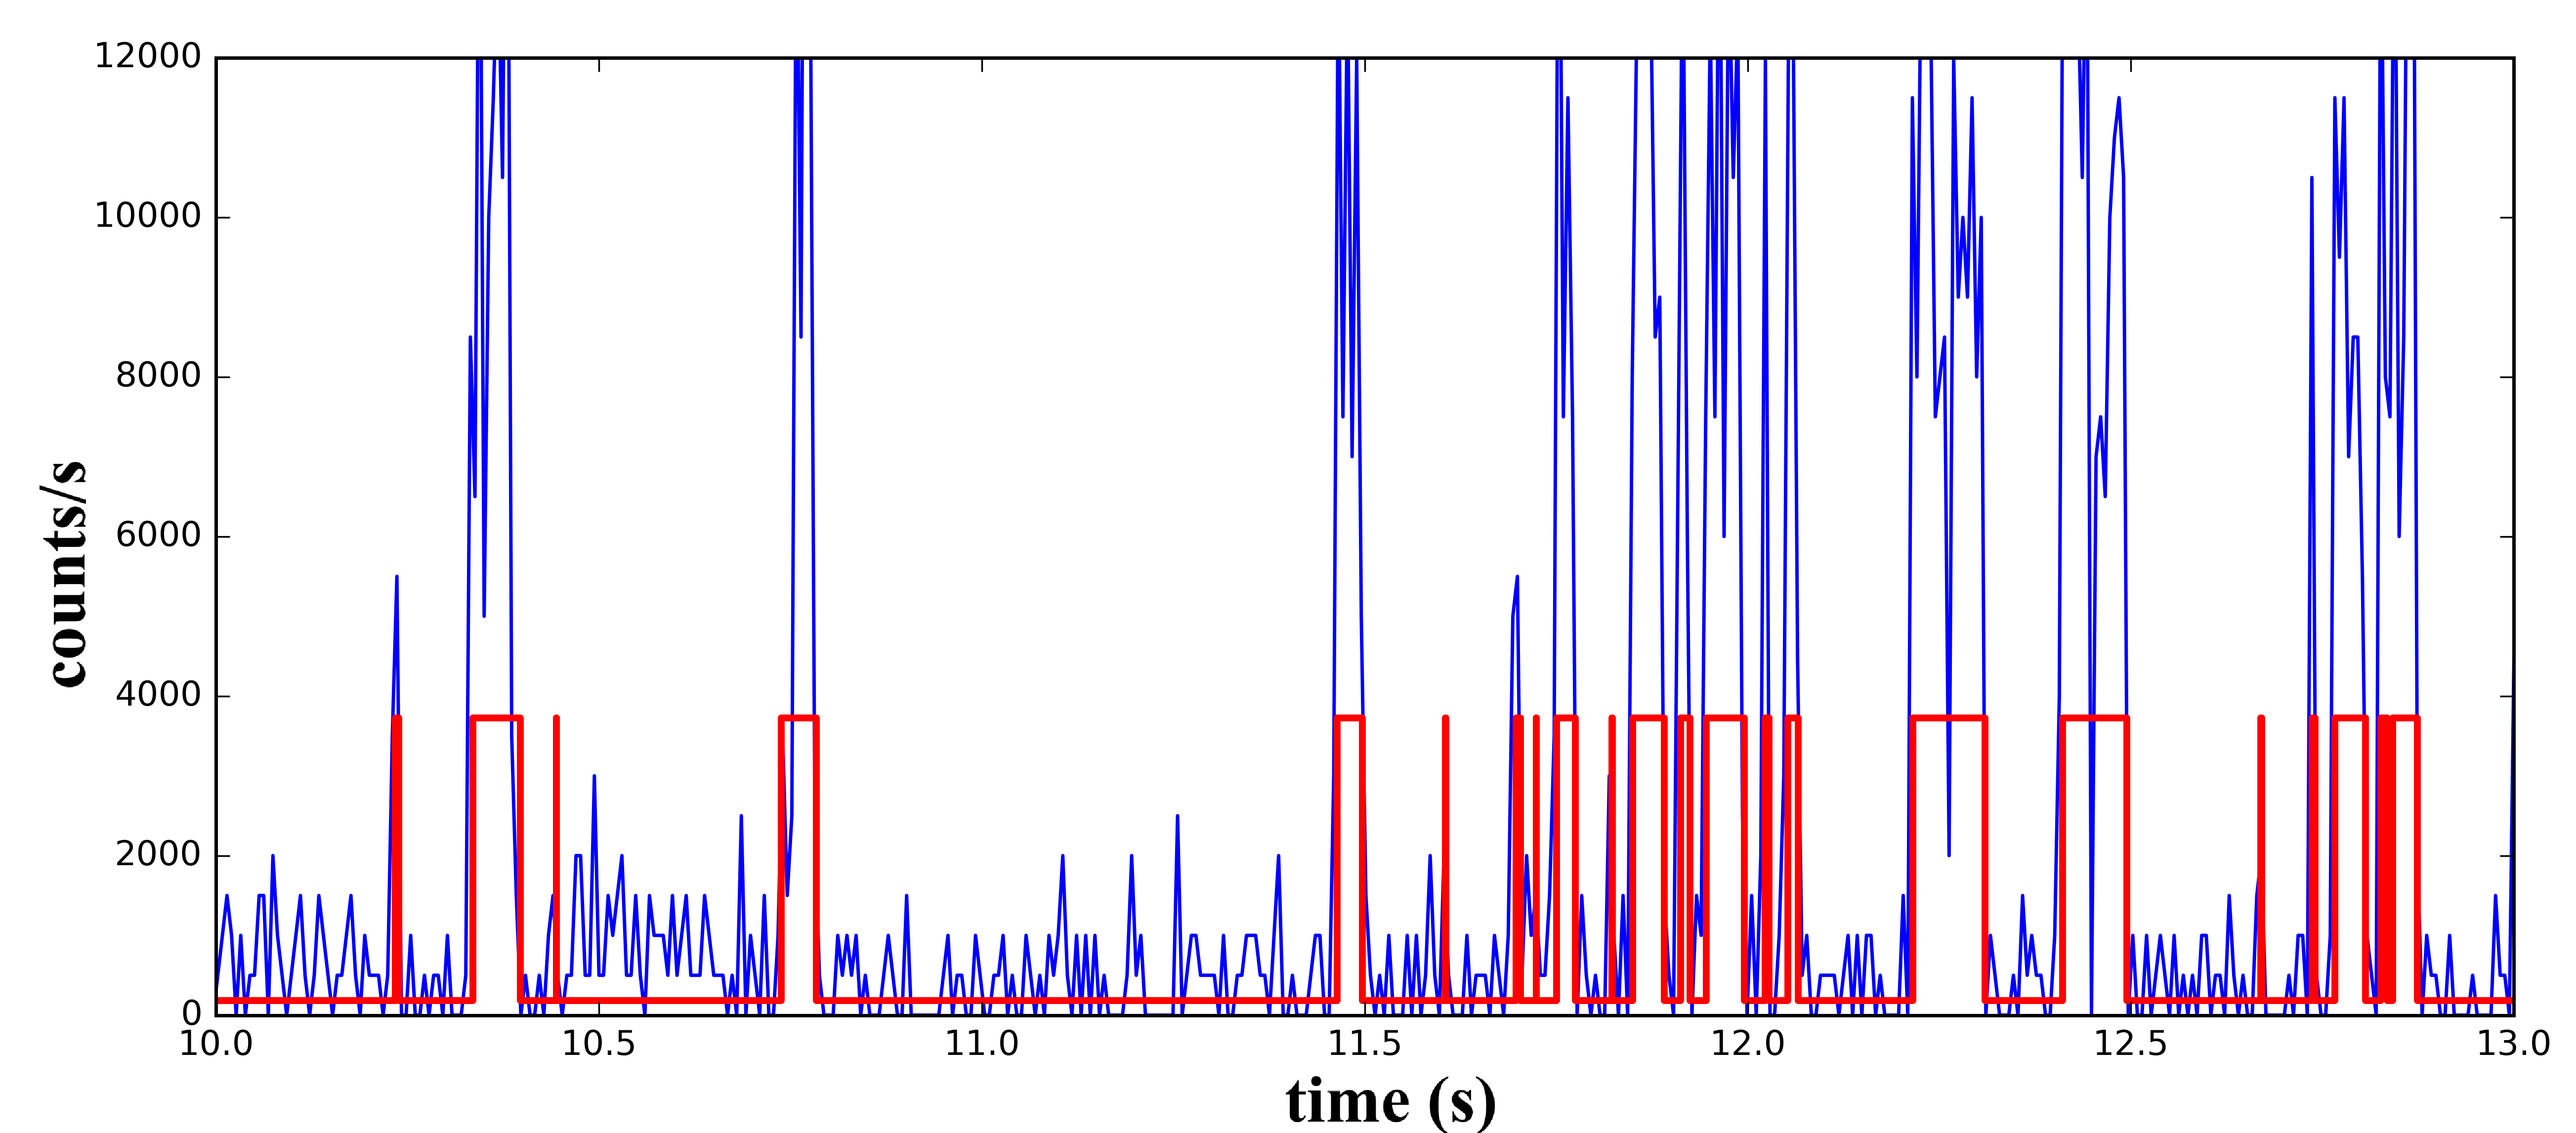
\includegraphics[width= \textwidth]{tt.png}
\caption{Example of a small part of a 30 sec timetrace of an immobilized Cu-Azurin in a 100 mV potential, taken with a CLSM. The blue line is the raw data, the red line is the fitted on and off magnitude and changepoint times. This is calculated using a specific program which is in more details described in the section \ref{dats_colls}.} 
\label{TT_exam}
\end{figure}

\section{Binding protein to the surface}\label{neutra}
In a variety of different applications, such as detection systems, the biotin-avidin system has been used \cite{Diamandis1991}. Living organisms develop highly specific defence mechanisms to help survive in unfriendly environments. Avidin, a protein found in egg white, has the ability to bind with very high affinity to vitamin biotin. This interaction is thought to represent a natural defence mechanism: the binding of avidin with biotinylated enzymes inactivates the enzymes that participate in $\textup{CO}_{2}$ transfer and thus inhibits the growth of bacteria. Compared to other  ligand-binder interactions, biotin-avadin has unique characteristics. The nonconvalent interaction of avadin with biotin has a formation constant of $10^{15}\textup{L}\cdot \textup{mol}^{-1}$, much greater than the interaction of ligands with their specific antibodies (about $10^{3}-10^{6}$ times greater). On top of that, the avidin possesses four binding sites per molecule. 

The NeutrAvidin is used unlabeled and serves as a link between the biotinylated binder (the biotin on the glass slide) and the biotinylated molecule (labeled Cu-azurin). This is illustrated in Figure \ref{avadinbinding} 

\begin{figure}[ht!]
\centering
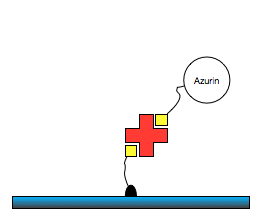
\includegraphics[width=70mm]{avadin}
\caption{Illustration of the sample slide - NeutrAvidin - protein binding. The red cross is the NeutrAvidin, with the four corners representing the binding spots for biotin. The yellow squares represent the biotin. One side is bound to the glass surface while the other side is connected to the azurin}
\label{avadinbinding}
\end{figure}


\section{Oxidation-reduction reactions}
Electron transfer (ET) is the exchange of electrons between molecules and can be generated by movements of electrons from one molecule to another in an oxidation-reduction (redox) reaction. Oxidation is the loss of electrons, reduction is the acquisition of electrons. The species being oxidized is called the reductant and the species being reduced is called the oxidant. The oxidation-reduction reaction can occur spontaneously. The two molecules participating in the electron transfer form a so called redox couple. The tendency to give or accept electrons is quantified by the midpoint potential which is generally measured with reference to the standard hydrogen electrode (SHE). The greater the midpoint potential difference between the redox couple, the greater is the driving force of the electrons. When a solution contains a mixture of reductants and oxidants, the solution potential can be given by the Nernst equation:
\begin{equation} \label{nernst}
E = E^{0} - \frac{RT}{nF} \ln Q
\end{equation}
or in terms of $\log_{10}$
\begin{equation}
E = E^{0} - \frac{0.0592}{n} \log_{10} Q
\end{equation}
where Q is the reaction quotient and $E^{0}$ the midpoint potential. For a reversible reaction (which is usually the case in redox reactions)
\begin{equation}
 \textup{aA + bB}\rightleftharpoons\textup{cC + dD}
\end{equation}
where a, b, c and d are the stoichiometric coefficients for the balanced reaction, we can calculate the reaction quotient using:
\begin{equation}
Q=\frac{\left [\textup{C}  \right ]^{\textup{c}}\left [\textup{D}  \right ]^{\textup{d}}}{\left [\textup{A}  \right ]^{\textup{a}}\left [\textup{B}  \right ]^{\textup{b}}}.
\end{equation}
When the reaction is in equilibrium, the reaction quotient $Q$ is constant and equal to the equilibrium constant $K$. The equilibrium constant is related to the Gibbs free energy change of the reaction via the equation
\begin{equation}
\Delta G =  nF \Delta E .
\end{equation}


\section{Electrochemical detection}
Electrochemical detection instruments can be used for monitoring the current passing through a flow cell in liquid electrochemistry and flow injection analysis, but they can also be used for other electroanalytical applications. The potential control range of these instruments is $\pm10V$. To reach certain potentials, a constant potential is applied and the current is recorded as a function of time (amperometric i-t curve), as is shown in Figure \ref{amp_curve}. Once the current in the i-t Curve is constant (i.e the curve is flat), the solution has reached the demanded potential. 

\begin{figure}[ht!]
\centering
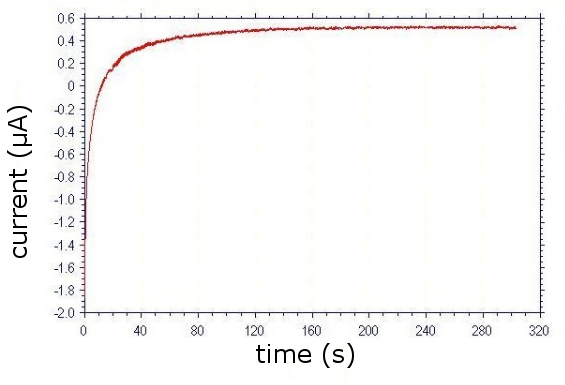
\includegraphics[width=.95 \linewidth]{it100mV}
\caption{The amperometric i-t of oxidizing conditions (100mV). The curve goes flat within minutes allowing a change in potential in relatively short times.}
\label{amp_curve}
\end{figure}



\chapter{Experimental setup}

This chapter covers the building of the setup from the start till the end. In papers and publications, it is not  common to describe how the experiment was built from the start till the end, but considered the duration and effort it took during this project it cannot be excluded from this thesis. The chapter is divided into three parts: the first part describes the setup in which the potential was tuned chemically by increasing or decreasing the concentration of  electron donor. This was the setup that was used previously to perform similar experiments with single molecules. The second part of this chapter covers the establishment of the electrochemically setup. The final part of this chapter discusses this setup and how it operates. It is this setup with which the data were acquired.

Some parts and techniques such as the confocal microscope and functionalizing of the glass slides are used in both setups. Therefore these are described below.

In this chapter and the rest of the thesis, the blue copper azurin used in the experiments is  labeled with ATTO 655 at binding site K122 (lysine at position 122). When copper azurin (CuAz) is mentioned, it is referred to the one with ATTO 655 label.
The potentials measured and mentioned in this thesis are always with respect to the calomel electrode and have a pH = 7.4 (unless otherwise specified).


\section*{Confocal microscope}  \label{confo_micro}
The experiments were performed on a home-built confocal microscope used for similar experiments. A 639 nm pulsed laser, controlled by a PDL 800-B (PicoQuant) laser driver at 40 MHz repetition rate, was passed through a narrow band clean-up filter (LD01-640/8-25, Semrock). To collimate the beam to the desired diameter an aspheric lens of suitable focal length was used. The beam then got reflected via a dichroic mirror (ZT640RDC, Chroma) to the high numerical aperture (NA) oil immersion objective (1.4 NA, 100X oil, Zeiss). The stage on which the sample was mounted was controlled by a nanopositioning piezo element (P517.3CD, Physik Instrumente). The emission was collected and filtered through an emission filter (ET655LP, Chroma) and focused onto a 50 $\upmu \textup{m}$ pinhole to remove background. Once the beam got focused on the active area of a single-photon counting module (SPCM-AQR-14, Perkin Elmer) data acquisition was performed by a photon counting PC-board (TimeHarp 200 PicoQuant). A schematic setup is shown in Figure \ref{micros}.

\begin{figure}[ht!]
\centering
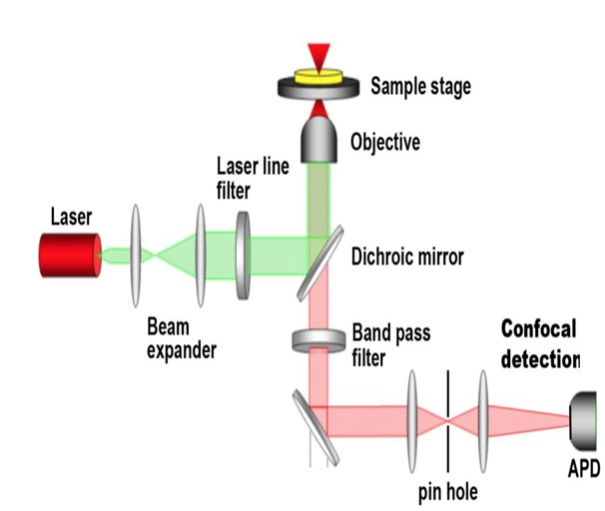
\includegraphics[width=.5\textwidth]{schem_micros}
\caption{Schematic drawing of the confocal microscope used in the chemical and electrochemical set up. }
\label{micros}
\end{figure}


\section*{Functionalizing glass slides}\label{functio}
The functionalization of the cover glass is based on the process used in similar experiments with immobilised molecules \cite{Gupta2014}\cite{Zimmermann2010}\cite{Hu2001}\cite{Halliwell2001}.  \diameter 25mm \#1 thickness glass coverslips (Menzel-Glaser) were used for all immobilizations. The coverslips were rinsed several times with milliQ water and treated with a  $\textup{H}_{2}\textup{O} / \textup{NH}_{4}\textup{OH} / \textup{H}_{2}\textup{O}_{2}$ (5:1:1) bath at 70$^{\circ}$ C. The coverslips were then rinsed again but with water and finally with ethanol. As a result of this process, the coverslips contain active hydroxyl groups. Before usage, the coverslips were flamed and then ozone-cleaned for 15 minutes. Then the coverslips were treated for 30 min with a 1\% solution of [3-(2-aminoethyl)aminopropyl]trimethoxysilane in methanol containing 5\% glacial acetic acid. This results in the binding of the active hydroxyl groups to the [3-(2-aminoethyl)aminopropyl]trimethoxysilane (step 1 in Figure \ref{func}). The silane is not yet covalently bound. This is obtained by removing the layer of water which stabilizes the interaction of silane with the hydrogen bonds. The water is removed by baking the coverslips in an oven at 65$^{\circ}$ C for 3 hours. After this treatment, the cover slips were sonicated for 10 minutes and washed with methanol. Dried with clean nitrogen, they were left in the desiccator overnigh. The next day they were treated with a mixture of 5 mg/mL methoxy-peg-N-hydroxysuccinimide (MW 2000, Laysan Bio) and 0.05 mg/mL biotin-peg-N-hydroxysuccinimide (MW 3400, Laysan Bio) in 50 mM phosphate buffered saline (PBS)  with pH 7.4 (step 2 in Figure \ref{func}). 
This creates the surface of biotin and methoxy. The biotin then will bind to the NeutrAvidin with the CuAz attached to it (see section \ref{neutra}). 

\begin{figure}[ht!]
\centering
\includegraphics[width=.3\textwidth]{funct_sampleslide}
\caption{Steps of the functionalizing of the glass coverslips. The active hydroxyl groups react with the [3-(2-aminoethyl)aminopropyl]trimethoxysilane resulting in hydrogen bonds (step 1). The N-hydroxysuccinimide (NHS) of the biotin/methoxy-peg-NHS mixture binds with the amino (step 2). The result is a surface with a 1:100 ratio of biotin to methoxy.}
\label{func}
\end{figure}


\section{Changing the potential chemically}\label{pot_chem}

A small glass slide is functionalized in a similar way as explained in section \ref{functio}. A syringe is used to suck solution through the tubes in a small cell onto the glass slide. One side is connected to the syringe, the other side is connected to the desired solution. First a solution of CuAz, NeutrAvidin and HEPES (pH = 7, 20mM) is put on the glass slide. After sufficient time, the CuAz will bind to the glass slide and the unbound CuAz will be removed by washing the slide with HEPES (pH = 7). Once the unbound proteins are removed, a new mixture containing 20mM ascorbate ($\textup{C}_{6}\textup{H}_{8}\textup{O}_{6}$) and 20mM potassium ferricyanide ($[\textup{Fe(CN)}_{6}]^{4-}$) is incubated into the flow cell. Ascorbate is an antioxidant and exists predominantly as the ascorbate monoanion  $\textup{AscH}^{-}$. The standard potential of ascorbate is around 40 mV (pH = 7) \cite{Creutz1981} with respect to a calomel electrode, which is close to the standard potential of CuAz. Oxidation of ascorbate forms $\textup{ascorbyl radical Asc}^{\bullet  -}$, the equivalent of ascorbate but with one less proton and one less electron. Upon further oxidation this becomes dehydroascorbate ($\textup{C}_{6}\textup{H}_{6}\textup{O}_{6}$) \cite{Warren2010}. This is schematically shown in Figure \ref{redox_asc}.

\begin{figure}[ht!]
\centering
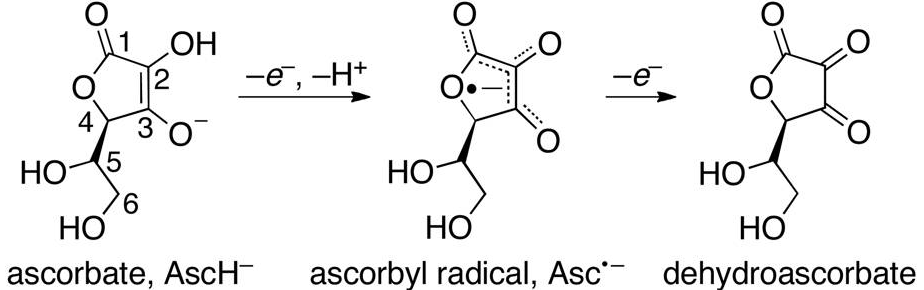
\includegraphics[width=\textwidth]{redox_asc}
\caption{Redox of ascorbate}
\label{redox_asc}
\end{figure}

At equilibrium, using the Nernst equation (Formula \ref{nernst}), the potential can be written as

\begin{equation}
E = E^{0} - \frac{RT}{nF} \ln \frac{[\textup{C}_{6}\textup{H}_{6}\textup{O}_{6}][\textup{Fe(CN)}_{6}]^{3-}}{[\textup{C}_{6}\textup{H}_{8}\textup{O}_{6}][\textup{Fe(CN)}_{6}]^{4-}}.
\end{equation}

Thus by adjusting the concentration of ascorbate (in this case adding ascorbate) or ferri-/ferrocyanide, different potentials will be achieved in the solution. The final redox potentials of the solution were measured with a reference electrode (standard calomel, SCE) and a platinum counter electrode connected to a voltmeter.

Some of the downsides to this setup are listed below:
\begin{itemize}
\item The change of potential is induced by adjusting the concentration of ascorbate or ferri/ferrocyanide. By adding or removing substances, the solution will be disturbed. The chance of losing the monitored proteins is substantial if this is not done carefully. 
\item Reaching specific potentials is only possible by adding or removing the exact amount of redox participants. A small mistake and the wanted potential will not be reached. 
\end{itemize}

These downsides lead ultimately to the desire of a better controllable and reliable setup. 

\section{Process to the final setup}

In the previous setup the potential was controlled by adding different amounts of chemicals. In the electrochemical setup, these changes are achieved electrochemically. Beside the confocal microscope, a new instrument has to be introduced: the electrochemical analyzer or potentiostat (Model 800B Series Electrochemical Detector, CH Instruments). Instead of using different concentrations of ascorbate, a cell with a working electrode, counter electrode and reference electrode in a buffer are used. During the process of getting to the final setup, the same working electrode, counter electrode and reference electrode is used: a \diameter0.25 mm gold wire acts as the working electrode, the counter electrode is a \diameter0.5 mm thin platinum wire and the reference electrode is a saturated calomel electrode. The SCE is based on the reaction between mercury and mercury(I) chloride. In adequous phase, saturated potassium chloride ($KCl$) in water is in contact with the mercury and the mercury(I) chloride. All the potentials throughout this work are reported relative to the SCE.

\subsection{Proteins on the surface}
Having functionalized sample slides and a fitting electron mediator, the next phase in the process to the final setup is to get the right amount of proteins on the sample slide. As mentioned in section \ref{neutra},  NeutrAvidin is used as a link between the sample slide and the proteins (see Figure \ref{avidinratio}). It has four possible binding spots  (Figure \ref{avidinratio}) and thus can bind up to four different CuAz via the $\textup{NH}_{2}$ groups on the CuAz.  Before the CuAz was applied on the sample slide, it was mixed with NeutrAvidin. Different ratios between the CuAz and NeutrAvidin were tried to find the right ratio. When the ratio between proteins and NeutrAvidin was 1:1, a shorter lifetime and lower intensity was observed for the immobilized proteins. This is because multiple CuAz would bind to the same NeutrAvidin. When more than one azurin is attached to the same NeutrAvidin, each azurin acts as a quencher to the other when close enough to each other \cite{Lakowicz2006}. The excited dye on one azurin can couple to the dye on the other azurin, which is attached to the same NeutrAvidin, resulting in quenching. The excited dye returns to the ground state, transferring its energy to the dye it is coupled to. Because of the short lifetime, this visualizes as blue spots on the lifetime image as is shown in Figure \ref{finding_proteins}. Lowering the ratio of proteins to the same amount of NeutrAvidin ensures the fact that less protein will bind to the same NeutrAvidin. At some point the probability that the NeutrAvidin is bound to more than one protein is very slim. This is the case when the ratio between protein and NeutrAvidin is 1:40 and this ratio is used in further experiments.

\begin{figure}[ht!]
\begin{subfigure}{.5\textwidth}

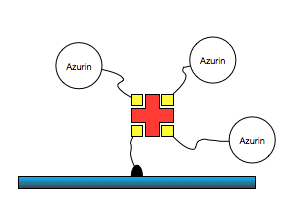
\includegraphics[width=70mm]{ratio_avadin}
\end{subfigure}%
\begin{subfigure}{.5\textwidth}

\includegraphics[width=.8\linewidth]{prot_neutr}
\end{subfigure}
\caption{Left: illustration of NeutrAvidin (red cross) bound to three azurin molecules via biotin (yellow). Right: the amide bond between biotin and azurin.}
\label{avidinratio}
\end{figure}


\begin{figure}
\begin{subfigure}{.5\textwidth}
  \centering
  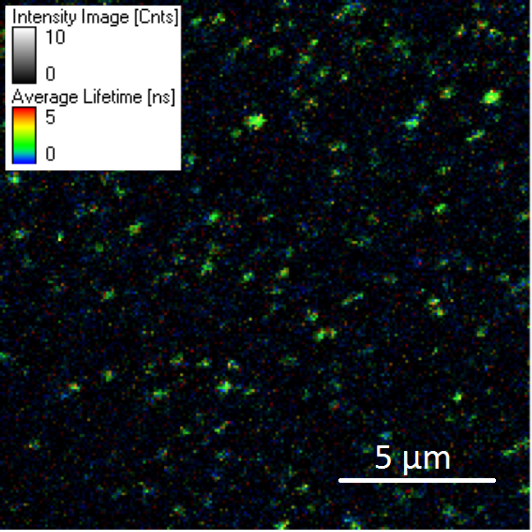
\includegraphics[width=.95 \linewidth]{onetooneratio}
  \label{}
\end{subfigure}%
\begin{subfigure}{.5\textwidth}
  \centering
  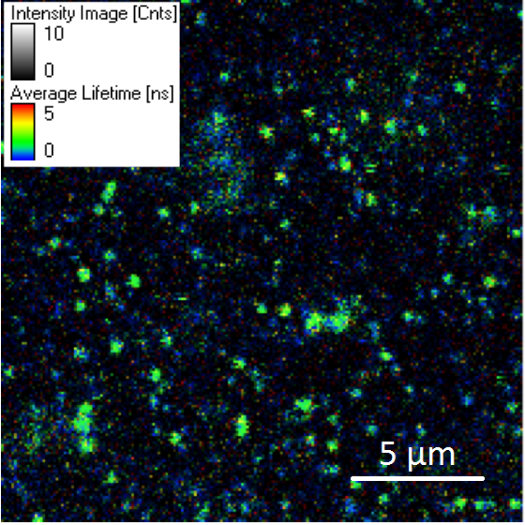
\includegraphics[width=.95 \linewidth]{onetofive}
  \label{}
\end{subfigure}
\caption{A (20 x 20) $\upmu \textup{m}^{2}$ lifetime image of immobilized azurin on the sample slide with different ratios of protein to NeutrAvidin at a potential of -100 mV. Left: the ratio between protein and NeutrAvidin is 1:1. Due to quenching, many CuAz are in dark state (short lifetime), but harder to see because of the background noise of the PES.  Right: the ratio between protein and NeutrAvidin is 1:5. When the amount of proteins to NeutrAvidin is decreased, a decreased amount of quenched CuAz is observed on the lifetime images.}
\label{finding_proteins}
\end{figure}


\subsection{The working electrode}
In an electrochemical system, the working electrode is the electrode of interest. In this case the working electrode is made of gold, since gold is one of the best electron conductors. The reaction of interest is occurring on and near the working electrode in conjunction with the counter electrode and reference electrode. Since the establishment of the redox potential relies on the diffusion of the electron mediator, the actual redox potential sensed by the molecule is dependent on the distance between the working electrode and the molecule as well as on the time after an external potential is applied. One way to keep the distance between the molecule and working electrode as small as possible is by creating a gold layer on top of the functionalized sample slides with the help a sputtering machine. After removing parts of the gold layer (creating transparent areas), the CuAz is applied on the sample slide. By creating transparent areas where proteins are immobilized such that the distance between the gold border and proteins is sufficient small and applying an external potential long enough, the potential on the gold is equal to the one in the near surrounding where the CuAz is immobilized. This gold layer is in touch with the potentiostat via a \diameter250 mm gold wire. Using a 20 nm thin gold layer gave a lot of problems, however.

One of the problems to overcome was to find a proper way to create transparent areas in the gold either by removing parts of the gold after the sputtering or by covering parts of the sample slide before sputtering so the gold can't reach certain areas. These areas need to meet requirements such as a size (usually a cross section of several tens of micrometer) big enough to monitor multiple (20-30) proteins at the same time.
Several different methods were tried (see Figure \ref{gold_layer}) and some of them are described hereafter.
\begin{enumerate}
\item \textbf{Scratches}.  The first attempt was sputtering the whole glass slide with a 20 nm thin layer of gold. With a needle scratches were made and imaged. When making scratches it is of big importance to not cross other scratches. Once the scratches cross each other, areas of gold that are isolated from the gold layer that is in touch with the wire can be created. The gold will not be connected to the working electrode in that case and no electrochemical changes will be seen near those edges. Once the scratches were made and put under the microscope it was easy to locate the areas where the gold was removed. However, these transparent areas were often too small to monitor multiple proteins at once. Beside that, the functionalized sample slide happened to get damaged along this process: when making scratches it is difficult to apply the same pressure along the scratches resulting in different depth of scratches. The dimension of proteins are in the nanometers. Different depths make it impossible to focus on multiple proteins in the same area at once.
\item \textbf{Small pieces of glass}. To get areas with the same depth, small pieces of smashed glass were laid on top of the functionalized glass slide before sputtering with gold. Once the sputtering was finished, the pieces of glass were removed resulting in small transparent areas (see the left side of Figure \ref{gold_layer}). The borders between glass and gold were sharp (the borders were 'sharp' on the images), but again a lot of areas formed via this method were too small to monitor multiple proteins. Later it was done with only a few bigger pieces of glass to avoid these small areas. This showed some improvement. 
\item \textbf{Metal crosses.} Small metal crosses on top of the glass before sputtering, resulting in cross-like transparent areas (see Figure \ref{gold_layer}). These transparent areas were easy to locate, the edges were straight and the borders were sharp as long as the gold layer was 30 nm thick, see Figure \ref{border}. If a certain (80 x 80) $\upmu \textup{m}^{2}$ area didn't suit single protein experiments, it is easy to slide along the border to find an area that suits better. 
\end{enumerate}

\begin{figure}
\begin{subfigure}{.5\textwidth}
  \centering
  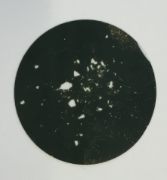
\includegraphics[width=.7\linewidth]{glass}
  \label{cross}
\end{subfigure}%
\begin{subfigure}{.5\textwidth}
  \centering
  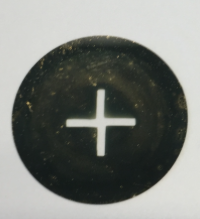
\includegraphics[width=.7\linewidth]{cross}
  \label{glass}
\end{subfigure}
\caption{A few examples of the \diameter 25 mm glass slides with a gold layer on top of it. Left: the transparent areas created with the help of small pieces of glass. Right: with the use of small iron crosses a cross-shaped transparent area was created.}
\label{gold_layer}
\end{figure}

\begin{figure}[ht!]
\centering
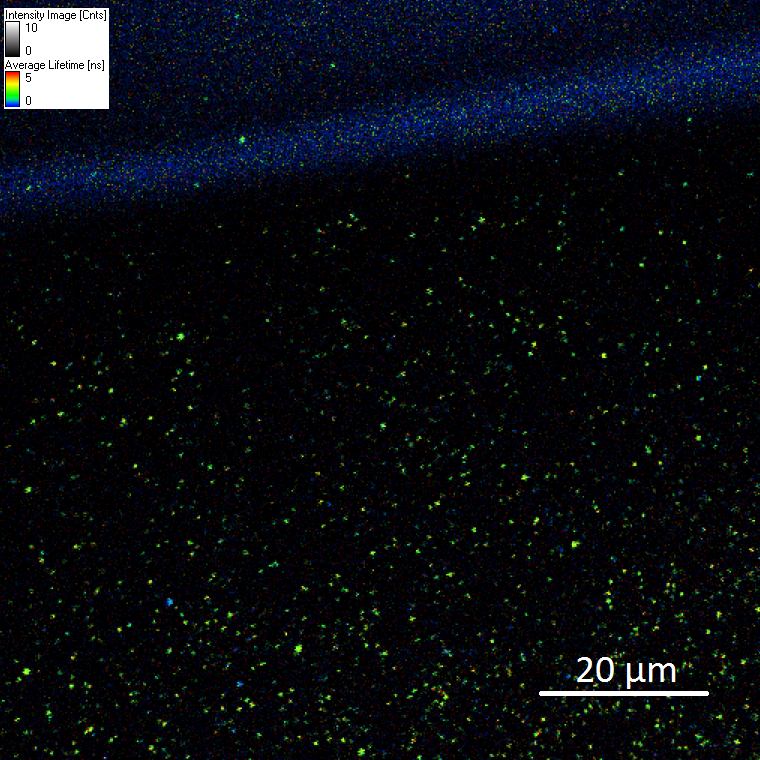
\includegraphics[width=\textwidth]{border_legenda}
\caption{(80 x 80) $\upmu \textup{m}^{2}$ image of the sharp border. The top part of the image is gold, the bright blue line is the border between the gold and the glass and the green spots below the border are azurin single molecules.}
\label{border}
\end{figure}

The latter method to create reliable areas is used in the next phase of the experiment: the combination of the electron mediator, proteins and the gold layer. Individually these parts worked as intended. However, a combination of the parts led to two serious problems:
\begin{enumerate}


\item Damaged gold layer.
The longer the experiment continued, the more clear it was that the border of the gold layer got slowly damaged. At the end of a day of experiments, the gold layer was damaged to such an extent that it would simply detach from the sample slide. This is a big problem since the distance between the border of gold/glass and the CuAz has to be minimized. The PES is most likely the reason for this. Though the exact reason for this was never clear - when a gold layer was exposed to a different electron mediator (ferricyanide or ascorbate) the gold layer was not damaged. The damage caused by PES can be seen if you compare the border of the gold layer (bright blue) of Figure \ref{no_prot} (left) - taken at the start of the experiment -  with the border of Figure \ref{no_prot} (right side, this picture was taken towards the end of a day of experiments). One way to tackle this problem would be a protective layer on top of the gold layer. This protective layer is 4-mercaptobutanoic acid ($\textup{C}_{4}\textup{H}_{8}\textup{O}_{2}\textup{S}$). This kind of protective layer has been used in similar experiments \cite{Elmalk2012} where it has been shown that the length of the carbon chain can vary without affecting the electron exchange between the gold and the single molecule. In these experiments, however, usually the molecules were on top of the gold layer whereas in our case the proteins are next to the gold layer. The result of using this protective layer was that the proteins did not show any reaction to a change in potential. Since the protective layer did not work, the other way to tackle the damaged gold layer is an increase in thickness of the gold layer. This will not prevent the PES from damaging the gold layer, but the process will be delayed long enough to perform experiments for a day. In all previous experiments, the thickness of the gold layer was 20 nm. Increasing the thickness of the gold layer to 200 nm led to the second problem, however.


\begin{figure}[ht!]
\centering
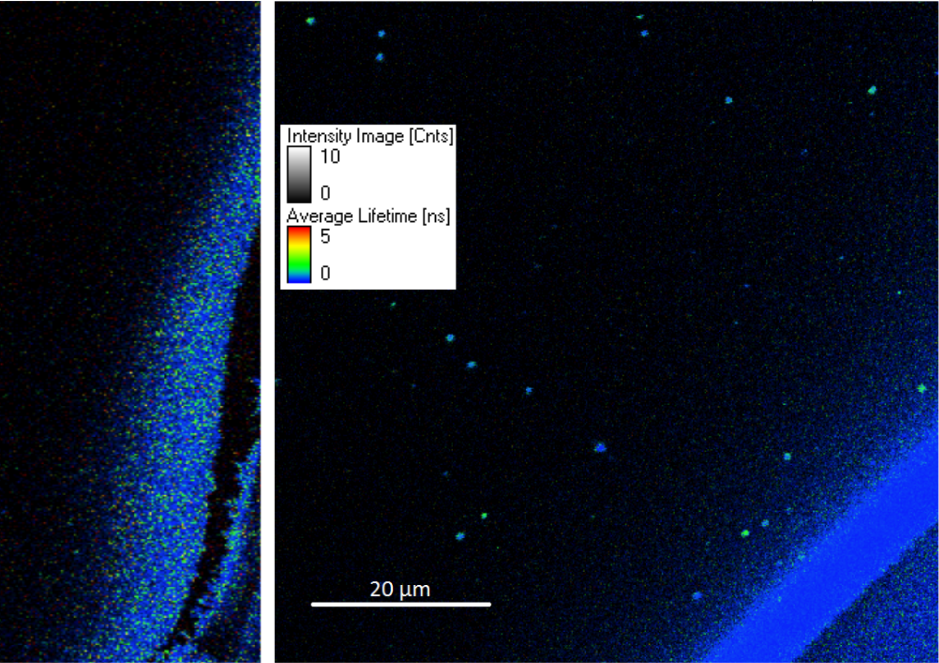
\includegraphics[width=\textwidth]{no_prot_damaged_border}
\caption{Left: part of an (80 x 80) $\upmu \textup{m}^{2}$ area showing the fractured gold border (bright blue) due to PES damaging the gold layer. Right: the (80 x 80) $\upmu \textup{m}^{2}$ of the glass surface near the 200nm thick gold layer. The part above the blue bright gold border is the transparent glass slide, the bottom right side below the bright blue line is the gold layer. As can be seen, almost no proteins are present on the transparent part of the sample slide, despite using the same molecule density as in earlier experiments.}
\label{no_prot}
\end{figure}



\item Missing proteins.
Near the edges of the working electrode, a much lower density of proteins was observed (see Figure \ref{no_prot}) once the gold layer thickness was increased. The reason for this could be that during the sputtering of the gold layer, the metal crosses would slightly move a little bit and thus damage the methoxy-peg-NHS layer. This would make it harder for proteins to bind near the surface. Another explanation could be that some gold-atoms might have slipped under the metal cross and occupied the spots where the proteins usually would bind. 



\end{enumerate}

\subsection*{The final setup: platinum grid} \label{grid_1}
At this point it was clear that the gold-layer as a working electrode in the current setup gave too many problems and a different solution was attempted. Instead of using a gold layer, a single gold wire was kept on the sample slide to see if this would give any good results. This can be seen in Figure \ref{goldenwire_1}. The green color are the proteins showing switching and blinking. This was the first sign that instead of the gold layer, a (gold) wire on its own suited as a working electrode. Finding a single wire with the microscope and keeping it on the sample slide is a tough task and is not controllable and thus a change was needed. Instead of one gold wire, a platinum rectangular grid (the total length/width of the grid is around 2.5 cm) was used and pressed onto the sample slide with the help of a small glass slide. Not only is the pressure evenly applied on the grid when pressure is applied on the glass slide on top of the grid, but also small confined volumes are formed where the sample slide and glass slide form the 'floor' and 'roof' and the platinum grid the 'walls'. These confined volumes are in the order of nanoliters, which makes switching possible in a matter of minutes. On top of changing the working electrode, also the electron mediator was changed. Once the setup worked, PES showed more disadvantages such as its very high autofluorescence which makes the signal-to-noise ratio very low. PES is hydrophobic and is difficult to mix with the PBS: it will get stuck on the surface and interacts with the proteins. To avoid these problems a different electron mediator is used in the final experiments. A mixture of 200 $\upmu \textup{M}$ ferricyanide and 100 $\upmu \textup{M}$ ascorbate was mixed with PBS to a total volume of 4 mL. This was the last step in order to make the whole setup work as intended. The setup is schematically drawn in Figure \ref{final_setup} with a short description of its parts.


\begin{figure}[ht!]
\centering
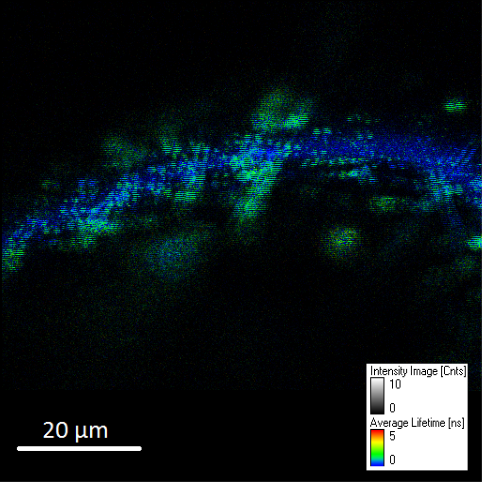
\includegraphics[width=\textwidth]{goldwire_1}
\caption{A (80 x 80) $\upmu \textup{m}^{2}$ area of the sample slide with immobilized proteins. The blue 'snake' is the gold wire that touches the sample slide. The green spots represent the reduced CuAz. This is the first sign that proteins near the wire show redox.}
\label{goldenwire_1}
\end{figure}


\begin{figure}[ht!]
\centering
\includegraphics[width=.75 \textwidth]{final_setup}
\caption{Not to scale schematic picture of the final setup in which the potential is changed electrically. \textbf{(1)} The confocal microscope as described at the beginning of this chapter. \textbf{(2)} The functionalized sample slide with on top the platinum grid and another small glass slide to press the grid on the sample slide, resulting in small confined volumes in the order of nanoliters. \textbf{(3)} The electron mediator consisting of 200 $\upmu \textup{M}$ ferricyanide, 100 $\upmu \textup{M}$ ascorbate and PBS (PH 7.4) with a total volume of 4 mL. \textbf{(4)} The working electrode (gold wire) in connection with the platinum grid (section \ref{grid_1}). \textbf{(5)} The saturated calomel reference electrode. \textbf{(6)} A platinum wire, not touching the grid, as the counter electrode. \textbf{(7)} The potentiostat ( Model 800B Series Electrochemical Detector, CH Instruments) to which the electrodes are connected. \textbf{(8)}, \textbf{(9)} Top view of the sample slide and two pictures of the same area showing the CuAz reduced and oxidized.}
\label{final_setup}
\end{figure}

\chapter{Results and discussion}

The experiments were performed with the blue copper protein azurin from \textit{Pseudomonas aeruginosa}, labeled with ATTO 655 (refered to as CuAz in the rest of the analysis). This small protein, with a molecular mass of 14 kDa, is involved in electron transfer (ET) reactions in a variety of bacteria. Its label, ATTO 655, has been chosen since its properties have been well documented \cite{pvd_11}. The labeling site used in this experiment is K122 (lysine at position 122), one of the close labeling sites to the copper center of CuAz.
Beside the blue copper protein azurin, fluorescently labeled zinc azurin (ZnAz) was also used to perform control experiments. Zinc azurin does not possess the ability to redox switch and is therefore an ideal control. When zinc azurin is exposed to different potentials, only the interactions between the dye and the solution change. By subtracting this interaction of the dye and the solution of the timetraces of CuAz, only the interaction between the electron mediators and the copper centre will remain. 

\section*{Data collection} \label{data_coll}
The sample, mounted on the scanning stages, was brought into the focal plane of the objective. Images of (10 x 10) ($\upmu \textup{m}^{2}$) were recorded as x-y scans. A positive and negative potential is applied to detect the redox switching CuAz. Images of typically (10 x 10) ($\upmu \textup{m}^{2}$) were recorded in which at least 10 redox switching molecules were present. To collect data from a single molecule, the laser was parked on the blinking molecule and measurements were made for 30 seconds.  Many fluorophores bleach within minutes, thus measurements of 30 seconds were chosen to increase the chance that the single molecule survive multiple potentials. Once all the blinking molecules of interest were measured at one potential, a new potential was applied and this process was repeated. Only the timetraces of those molecules who survived at least four different potentials were included for further analysis. 

To make sure that the surroundings of the single molecules were indeed at the intended potential, the I-t curves were recorded at the same time. Once the I-t curves stay constant, the solution has the same potential as the potentiostat applies. Two examples of these I-t curves are shown in Figure \ref{it_curves}

\begin{figure}[ht!]
\begin{subfigure}{.5\textwidth}
  \centering
  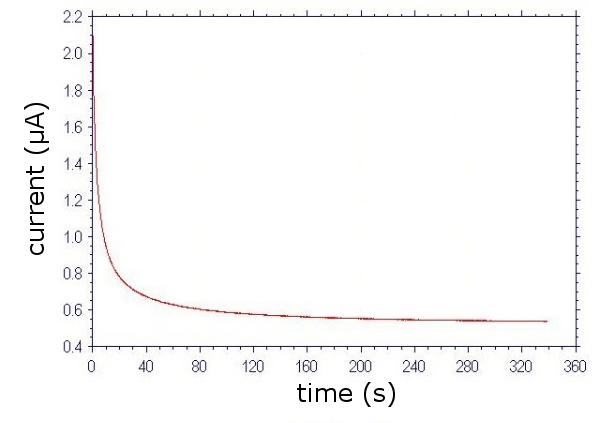
\includegraphics[width= \textwidth]{it25mV}

  \label{}
\end{subfigure}%
\begin{subfigure}{.5\textwidth}
  \centering
  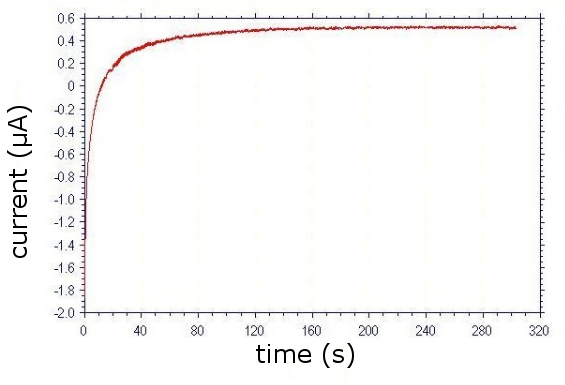
\includegraphics[width=.95 \linewidth]{it100mV}
  \label{}
\end{subfigure}
\caption{The amperometric I-t curve.  Left: the I-t curve of reducing conditions (-25 mV applied in this case). Right: the I-t curve of oxidizing conditions (100 mV applied in this case).}
\label{it_curves}
\end{figure}


\section*{Timetrace analysis}\label{dats_colls}
The software used for the fluorescence lifetime imaging and correlation software is SymPhoTime 64. With the help of this program, timetraces and their specific parameters are saved in .pt3 files. Older versions of SymPhoTime saved these data into .t3r files. Previous PhD student Dr. Ankur Gupta had written a program in MATLAB R2012b to read out the .t3r files and transfer the timetraces into multiple .dat files. This program has been adjusted in such a way that it can read out the .pt3 files from the newer version of SymPhoTime 64. It allows you to manually select parts of the timetrace, as is shown in Figure \ref{timetrace_selection}.

\begin{figure}[ht!]
\centering
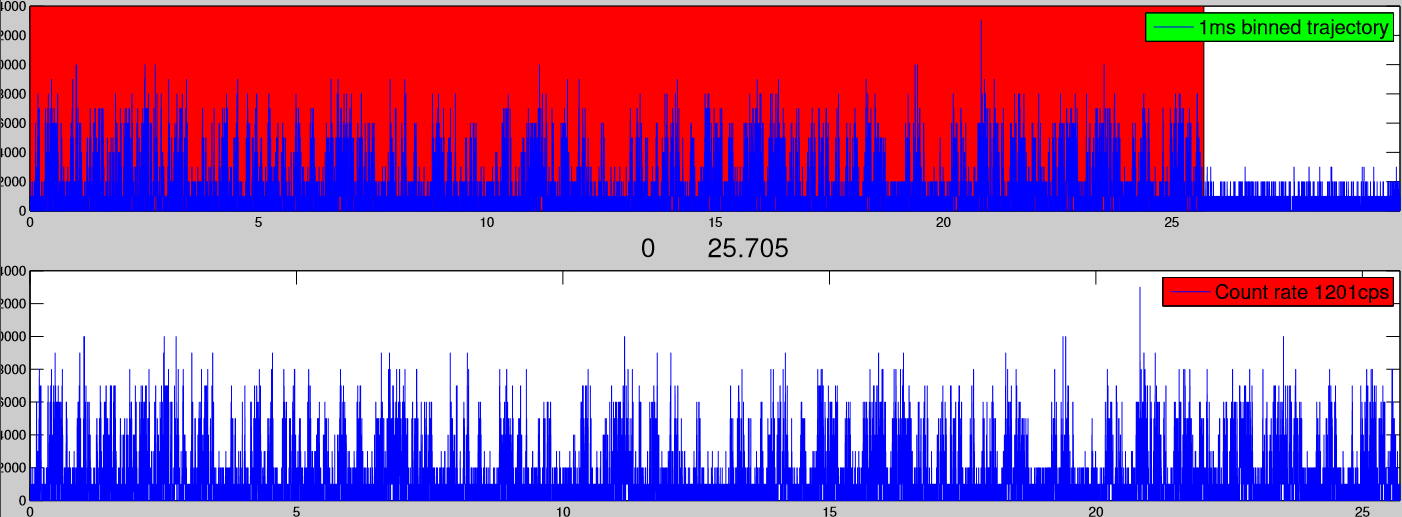
\includegraphics[width=\textwidth]{timetrace_selection}
\caption{Selection of a timetrace with a program written in MATLAB R2012b and C to select the parts of the timetrace (in red) that will be put into .dat files. In this specific case the CuAz bleached at around 25.7 s at a potential of 50 mV. Once the CuAz is bleached, the remainder of the timetrace is not of interest and thus not selected.}
\label{timetrace_selection}
\end{figure}

Once the timetrace is selected and put into several .dat files, another C program is run to precisely calculate the  on- ($\tau_{on}$) and off-times ($\tau_{off}$). This program uses several mathematical methods to identify the points in time where a discrete switch in intensity occurs. This is described in more detail by Lucas P. Watkins and Haw Yang in their paper \cite{And2004}. As an example, several on- and off times are visualized in Figure \ref{on_off_times}. The on-time is defined as the time when the intensity is high, which is the case when CuAz is reduced. The off-time is when the intensity is low and the CuAz is oxidized. The program does not distinguish the cause of the intensity jumps. In this case there are two main reasons for intensity jumps. The first reason is intensity jumps that are related to the redox of the copper center. These intensity jumps are referred to as 'switching'. The second reason is related to the (often) unwanted and uncontrolled intensity change due to the reaction between the dye and the redox chemicals in the solution. This is referred to as 'blinking'. To deduce the on- and off-times for the potentials where both switching and blink is present, the autocorrelation is used. This is explained in more detail in section \ref{autocor}.

\begin{figure}[ht!]
\centering
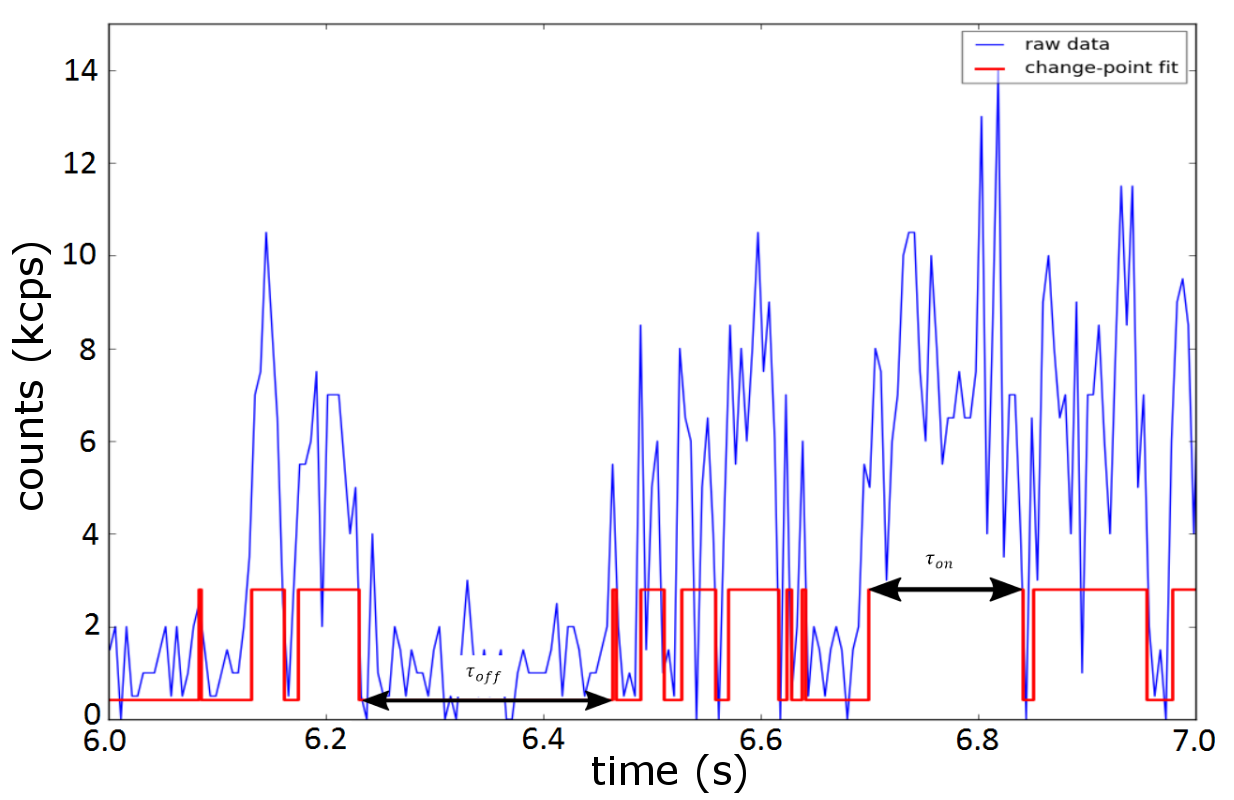
\includegraphics[width=\textwidth]{on_off_test1}
\caption{Same timetrace as Figure \ref{timetrace_selection} but a smaller range. In red is plotted the calculated intensity jumps according to the program written by Lucas P. Watkins and Haw Yang. The time when the intensity is low is referred to as the $\tau_{off}$ and the time the molecules intensity is high is the $\tau_{on}$.}
\label{on_off_times}
\end{figure}

\newpage


\begin{figure}[ht!]
\centering
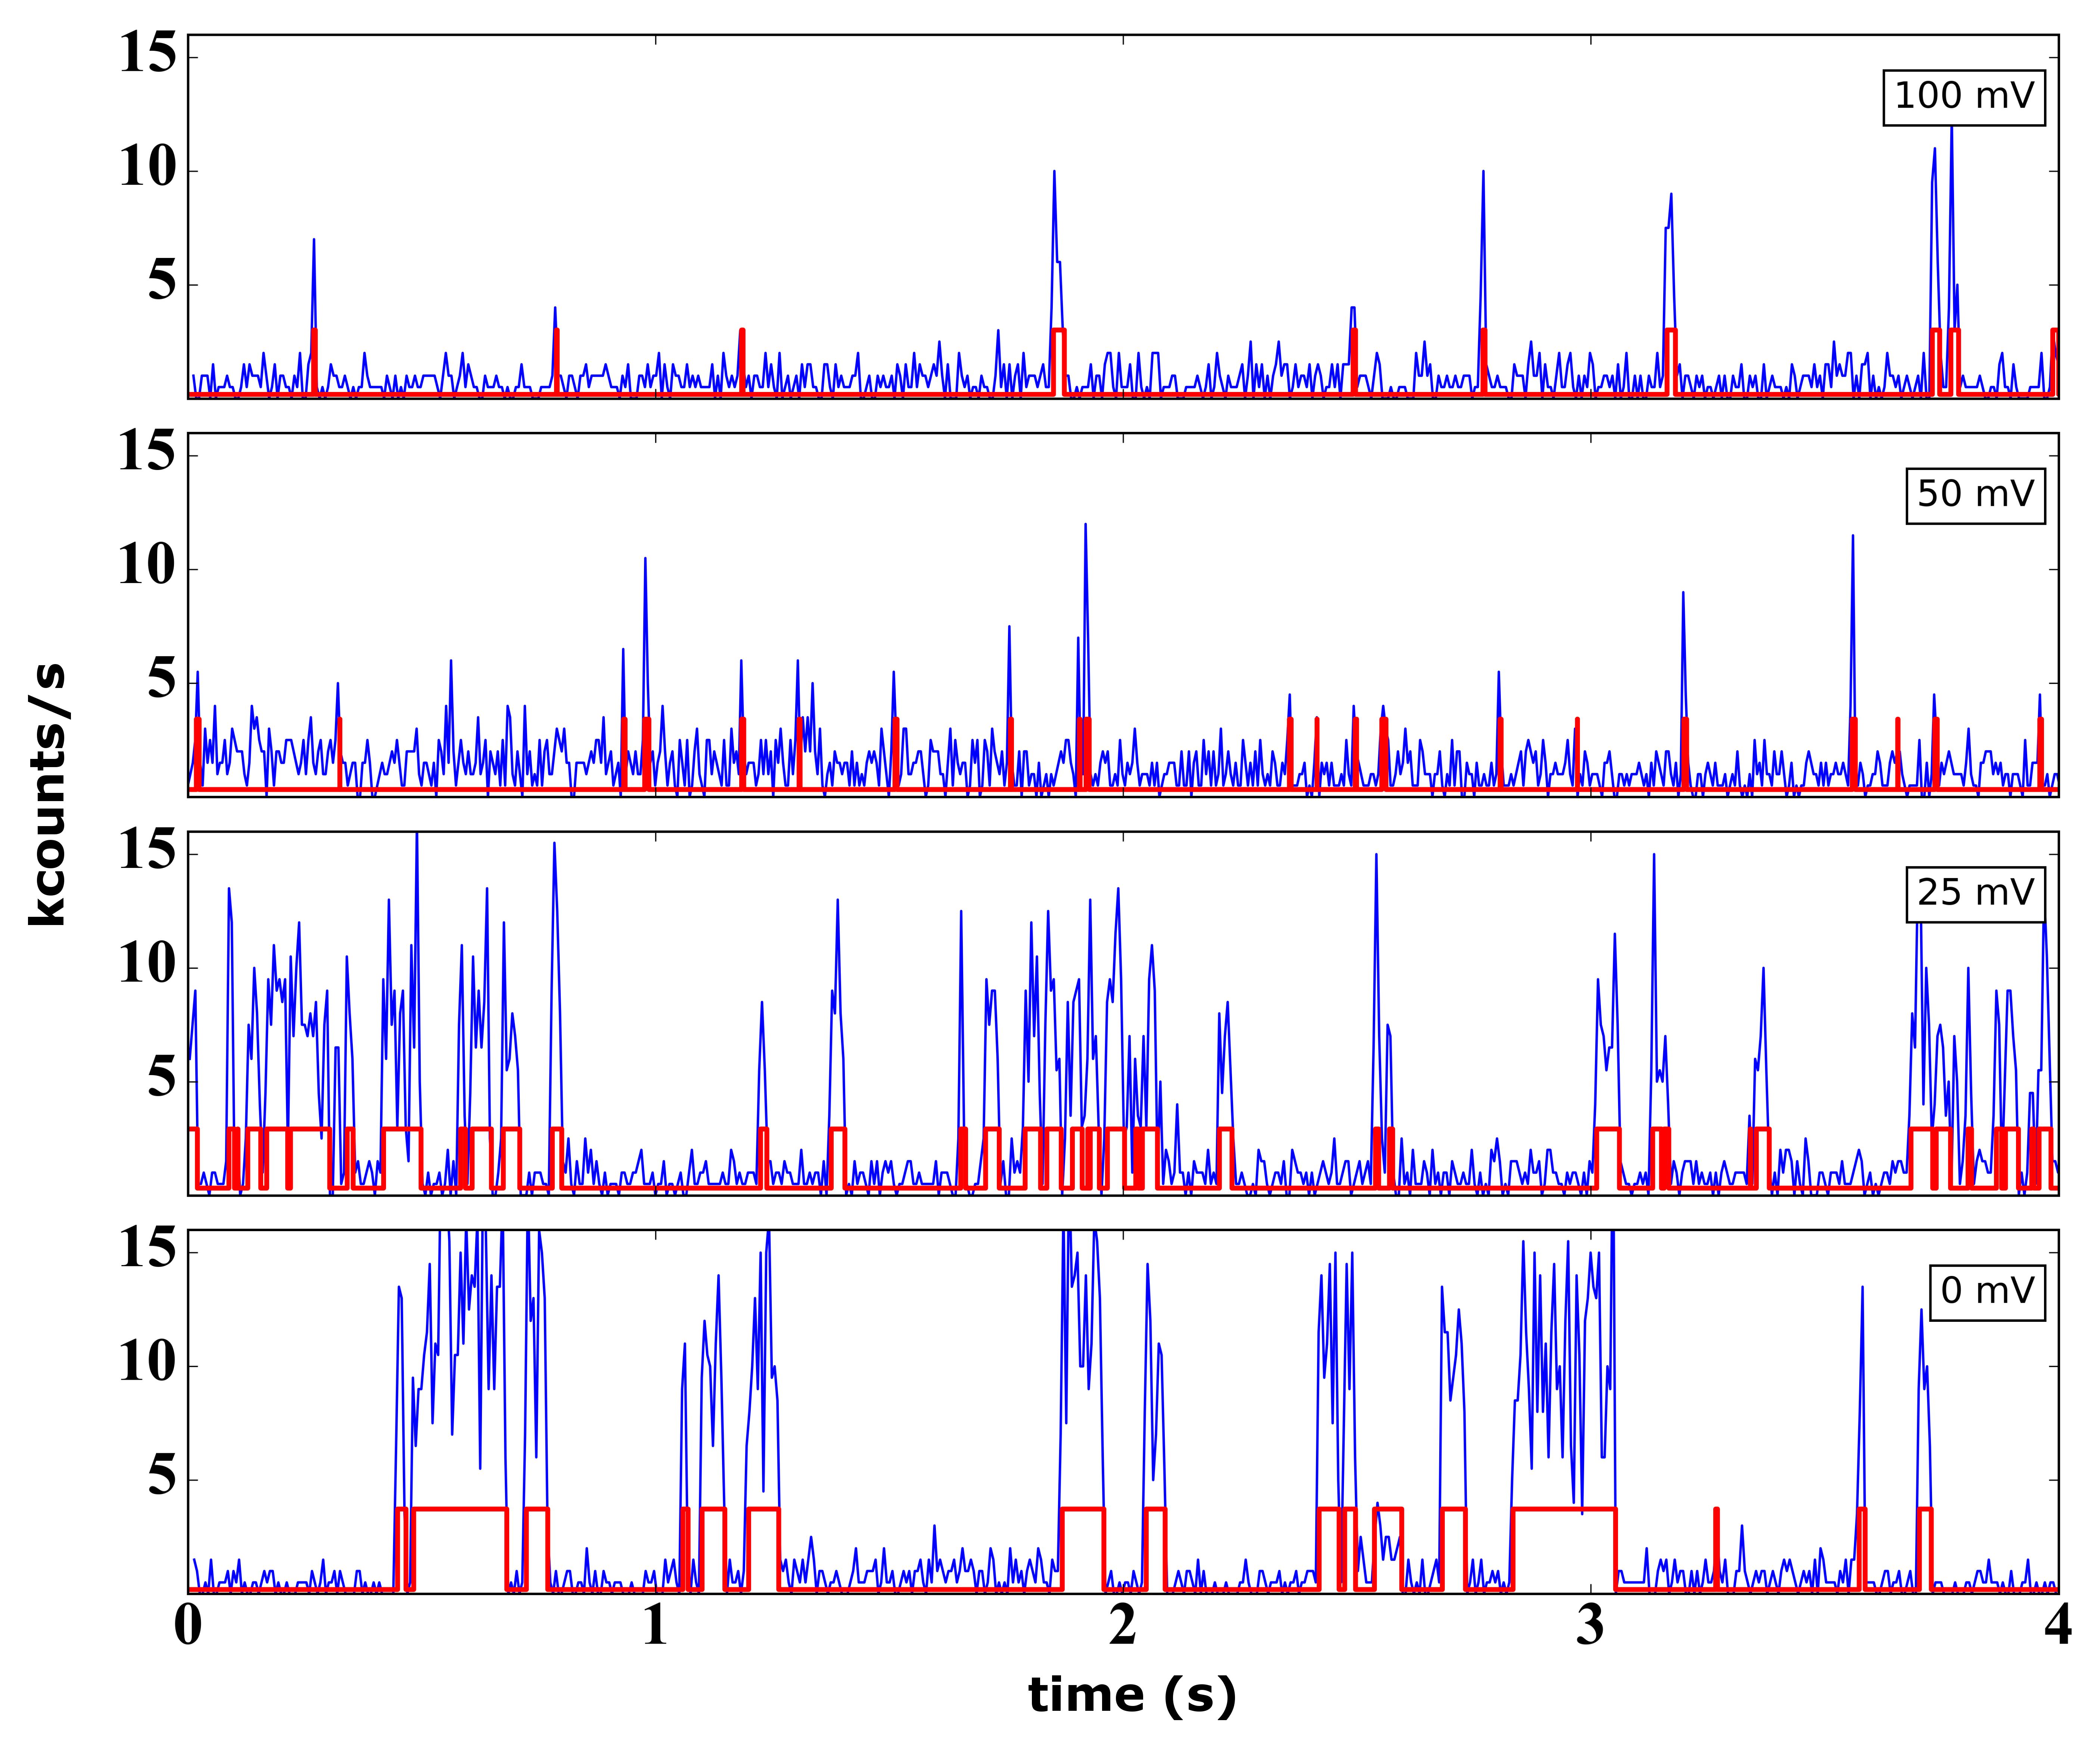
\includegraphics[width=1\textwidth]{plots_timetraces_diff_pot}
\caption{Timetraces (bin time is 10 ms) together with their autocorrelation of the same CuAz molecule under different potentials. A clear difference between $\tau_{on}$ and $\tau_{off}$ under different potentials is visible: shorter $\tau_{on}$ for higher oxidizing potentials, longer $\tau_{on}$ for reducing lower potentials. For potentials below 40 mV this pattern gets disturbed due to blinking of the ATTO 655.}
\label{plots_timetraces_diff_pot}
\end{figure}




\subsection{Timetraces CuAz}

Looking at the timetraces between 100 mV and 0 mV (Figure \ref{plots_timetraces_diff_pot}) a trend is noticeable. For the higher potentials, the off-times ($\tau_{off}$) are long and the on-times ($\tau_{on}$) are relatively short which goes hand in hand with the low amount of events and the low average fluorescence level. When the potential decreases, the amount of events start to increase and the $\tau_{on}$ becomes longer while $\tau_{off}$ becomes shorter. The explanation for this is simply the FluRedox principle. CuAz in oxidized form (copper is in $\textup{Cu}^{2+}$) shows an absorbance maximum around 628 nm which overlaps with the fluorescence emission of the ATTO 655 dye as is shown earlier in Figure \ref{absorption}. Since energy transfer is high in this form, the fluorescence of the dye is largely quenched resulting in longer $\tau_{off}$. When the potential is decreasing, the solution becomes more reducing. When CuAz is reduced - since the absorption at 628 nm disappears upon reduction - the energy transfer is low and thus the dye shows high fluorescence and longer $\tau_{on}$ times are expected. This mechanism seems to be the only one at work until the potential comes near 40 mV. Here a new phenomenon is noticeable (see the 25 mV and 0 mV timetraces in Figure \ref{plots_timetraces_diff_pot}). Beside the expected  increasing $\tau_{on}$ and decreasing $\tau_{off}$ due to switching of CuAz, a secondary timescale appears in the form of short $\tau_{on}$ in very short succession. To explain this event, a closer look has to be taken at the chemicals involved in the chemical processes concerning the redox reactions. Intermolecular reactions between the redox active components in the solution and the dye are present. For higher potentials, the timescale of the blinking events between dye and solution are long. When the potential gets lower, the solution is more and more reduced. The interaction between the dye and the reduced ascorbate and ferricyanide happens on a smaller timescale and is now prominent in the timetraces (see Figure \ref{plots_timetraces_diff_pot}). This is more apparent when looked at the autocorrelation: for the timetraces higher than 40 mV, the autocorrelation fits a single exponential. Below 40 mV, when the blinking of the dye - on top of the redox switching - is present, a biexponential fits the autocorrelation. More details on this in section \ref{autocor}.


Another way of looking at the on- and off-times acquired by the timetraces is by plotting the on- and off-times in histograms. This is done in Figure \ref{histograms_disc}. The on-times follow a single exponential distribution, but the off-times have a different form. Very short off-times seem to be relatively rare. The distributions of  $\tau_{on}$ and  $\tau_{off}$ should be both single exponential if the reduction and oxidation reactions are first order rate constants and involve only one rate constant. It has been shown previously that a simple two-step reaction
\begin{equation}\label{ox_pros}
\textup{A}{\overset{1}{\longrightarrow}\textup{B}\overset{2}{\longrightarrow}}\textup{C}
\end{equation}
predicts that the distribution of off-times is described by the difference between two exponentials \cite{Smiley2006}. These distributions have the same shape as the distributions of the off-times as can be seen in Figure \ref{histograms_disc} and the histograms are thus evident that the redox of copper involves two rate constants. To get a deeper understanding of this a closer look has to be taken at the electron transfer process between the solution and the copper azurin:
\begin{equation}\label{ox_pros}
\underset{\textup{\large low}}{\textup{Cu}^{2+} + \textup{R}} \overset{k_{1}}{\underset{k_{-1}}\rightleftarrows} \underset{\textup{\large low}}{\textup{Cu}^{2+}\textup{R}} \overset{k_{2}}\rightarrow \underset{\textup{\large high}}{\textup{Cu}^{+} + \textup{R}^{+}},  \qquad \underset{\textup{\large high}}{\textup{Cu}^{+}} \overset{k_{3}}\rightarrow \underset{\textup{\large low}}{\textup{Cu}^{2+}}.
\end{equation}
Here $k_{i}$ are the electron transfer rate constants and below each step is the intensity written. The reduction of $\textup{Cu}^{2+}$ to $\textup{Cu}^{1+}$ is a multi-step process if it is a predecessor-successor reaction. Bringing the electron close to the copper center (step 1) and reducing the copper (step 2) happens in two steps, characterized by the rates $k_{1}$ and $k_{2}$. \textbf{Therefore the reduction of copper involves two rate constants}. During these two steps, the intensity is low and results in the absence of short off-times. The oxidation of the copper  involves the removal of an electron from the center and is a single step process with rate $k_{3}$. This is consistent with the histogram of the on-times, which is mono exponential.

\begin{figure}[ht!]
\centering
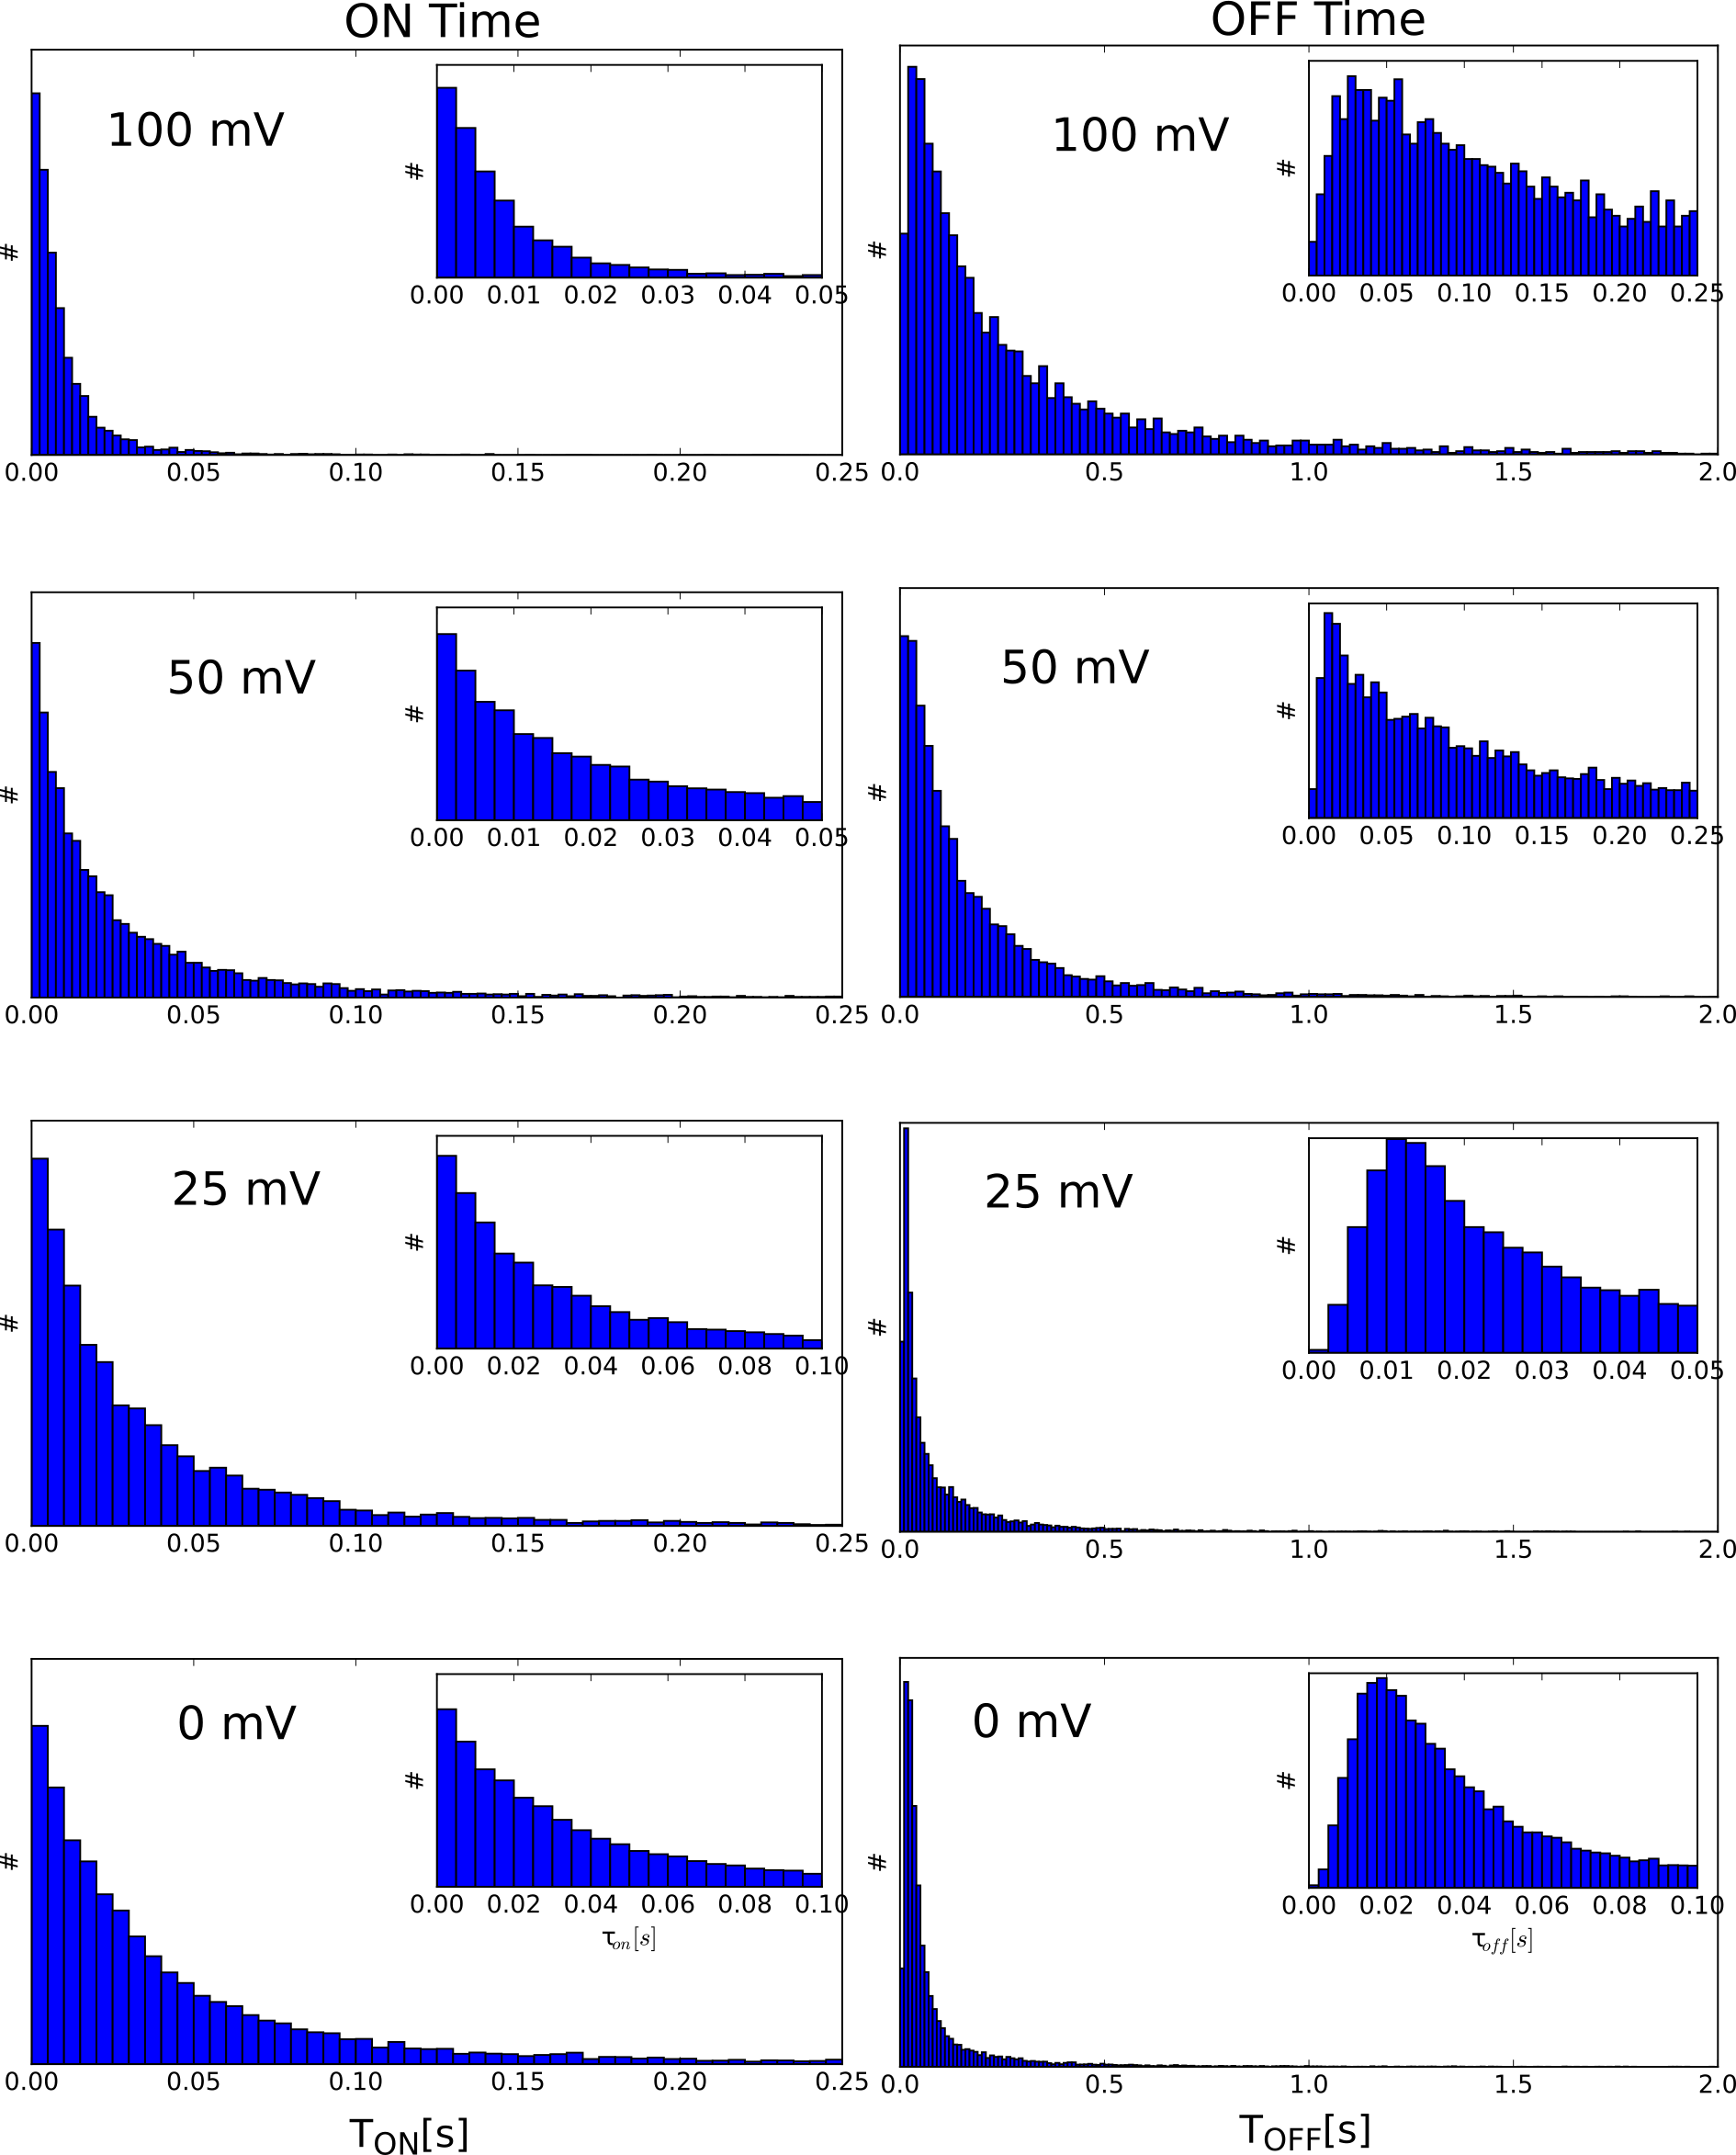
\includegraphics[width=.9\textwidth]{Figure_4_4_histogram_thesis}
\caption{Histogram distribution $\tau_{on}$ and $\tau_{off}$ of CuAz at different potentials.}
\label{histograms_disc}
\end{figure}

One feature of the on- and off-times histograms in Figure \ref{histograms_disc} is the fit through the histograms. The fit through the histograms allows the calculation of the electron transfer rates in equation \ref{ox_pros}. The mono-exponential fit through the on-time histograms will give the rate constant $k_{1}$, while a bi-exponential fit through the histograms of the off-times will lead to the rate constant $k_{3}$. This has been done previously in a similar experiment where they calculated the electron transfer rates  between the copper centers of a multicopper oxidase (MCO) using fits through the histograms \cite{Gupta2014a}. This is however not done for the data in this thesis, but is something that should be done in the future.

Finally we will look at the correlation of the on- or off-times after one or more turnovers. This has been done previously by M. Orrit et al. \cite{Lippitz2005}, where a simple fourstate system - in case of a first-order reaction - is proposed consisting of two two-level blinking models. This model is very similar to the case of CuAz, where the fast blinking and slow switching dominate the timetraces. Furthermore they showed that slow fluctuations lead to strong memory effects and the scatter plots follow inverse diagonals. When memory is completely absent (a random slow or fast blinking event for each cycle), a high number of correlation points is found where a short time correlates to a long one and vice versa (in other words: an excess of points near the axes). They have shown that for their timetraces, the memory is completely absent after 200 turnovers.
In our case, because of the short timetraces, the amount of events during these 30 s timetraces are typically around 180 turnovers (that is: 90 on-times and 90 off-times). Therefore, we are limited in our plots to a maximum of 40 turnovers. Here we shall discuss the outcome of two different cases of 31 single molecules:
\begin{itemize}
\item  The first case is at the potential of 100 mV and is shown in Figure \ref{on_plotjes}. Here, the blinking between the dye and the redox solution are minimal and the fluctuations are slow. The timetraces show strong memory effects after 20 and 40 turnovers for both the on- and off-times, though the off-times after 40 turnover show some signs of the memory effects becoming weaker, as more points are present on the axes (bottom right of Figure \ref{on_plotjes}). 
\item The second case is at 0 mV and is shown in Figure \ref{on_plotjes_2}. Here, the interaction between the dye and the solution predominate compared to the 100 mV potential. The off-time plots show - even after 1 turnover - absence of memory, as an excess of points on the axes is present. This absence becomes stronger when we increase the amount of turnovers to 40. 
\end{itemize}
With longer timetraces it is possible to plot the correlation after more turnovers and determine if and when the memory effects are completely absent, even for the timetraces of single molecules at 40 mV or higher potentials.


\newpage


\begin{figure}[ht!]
\centering
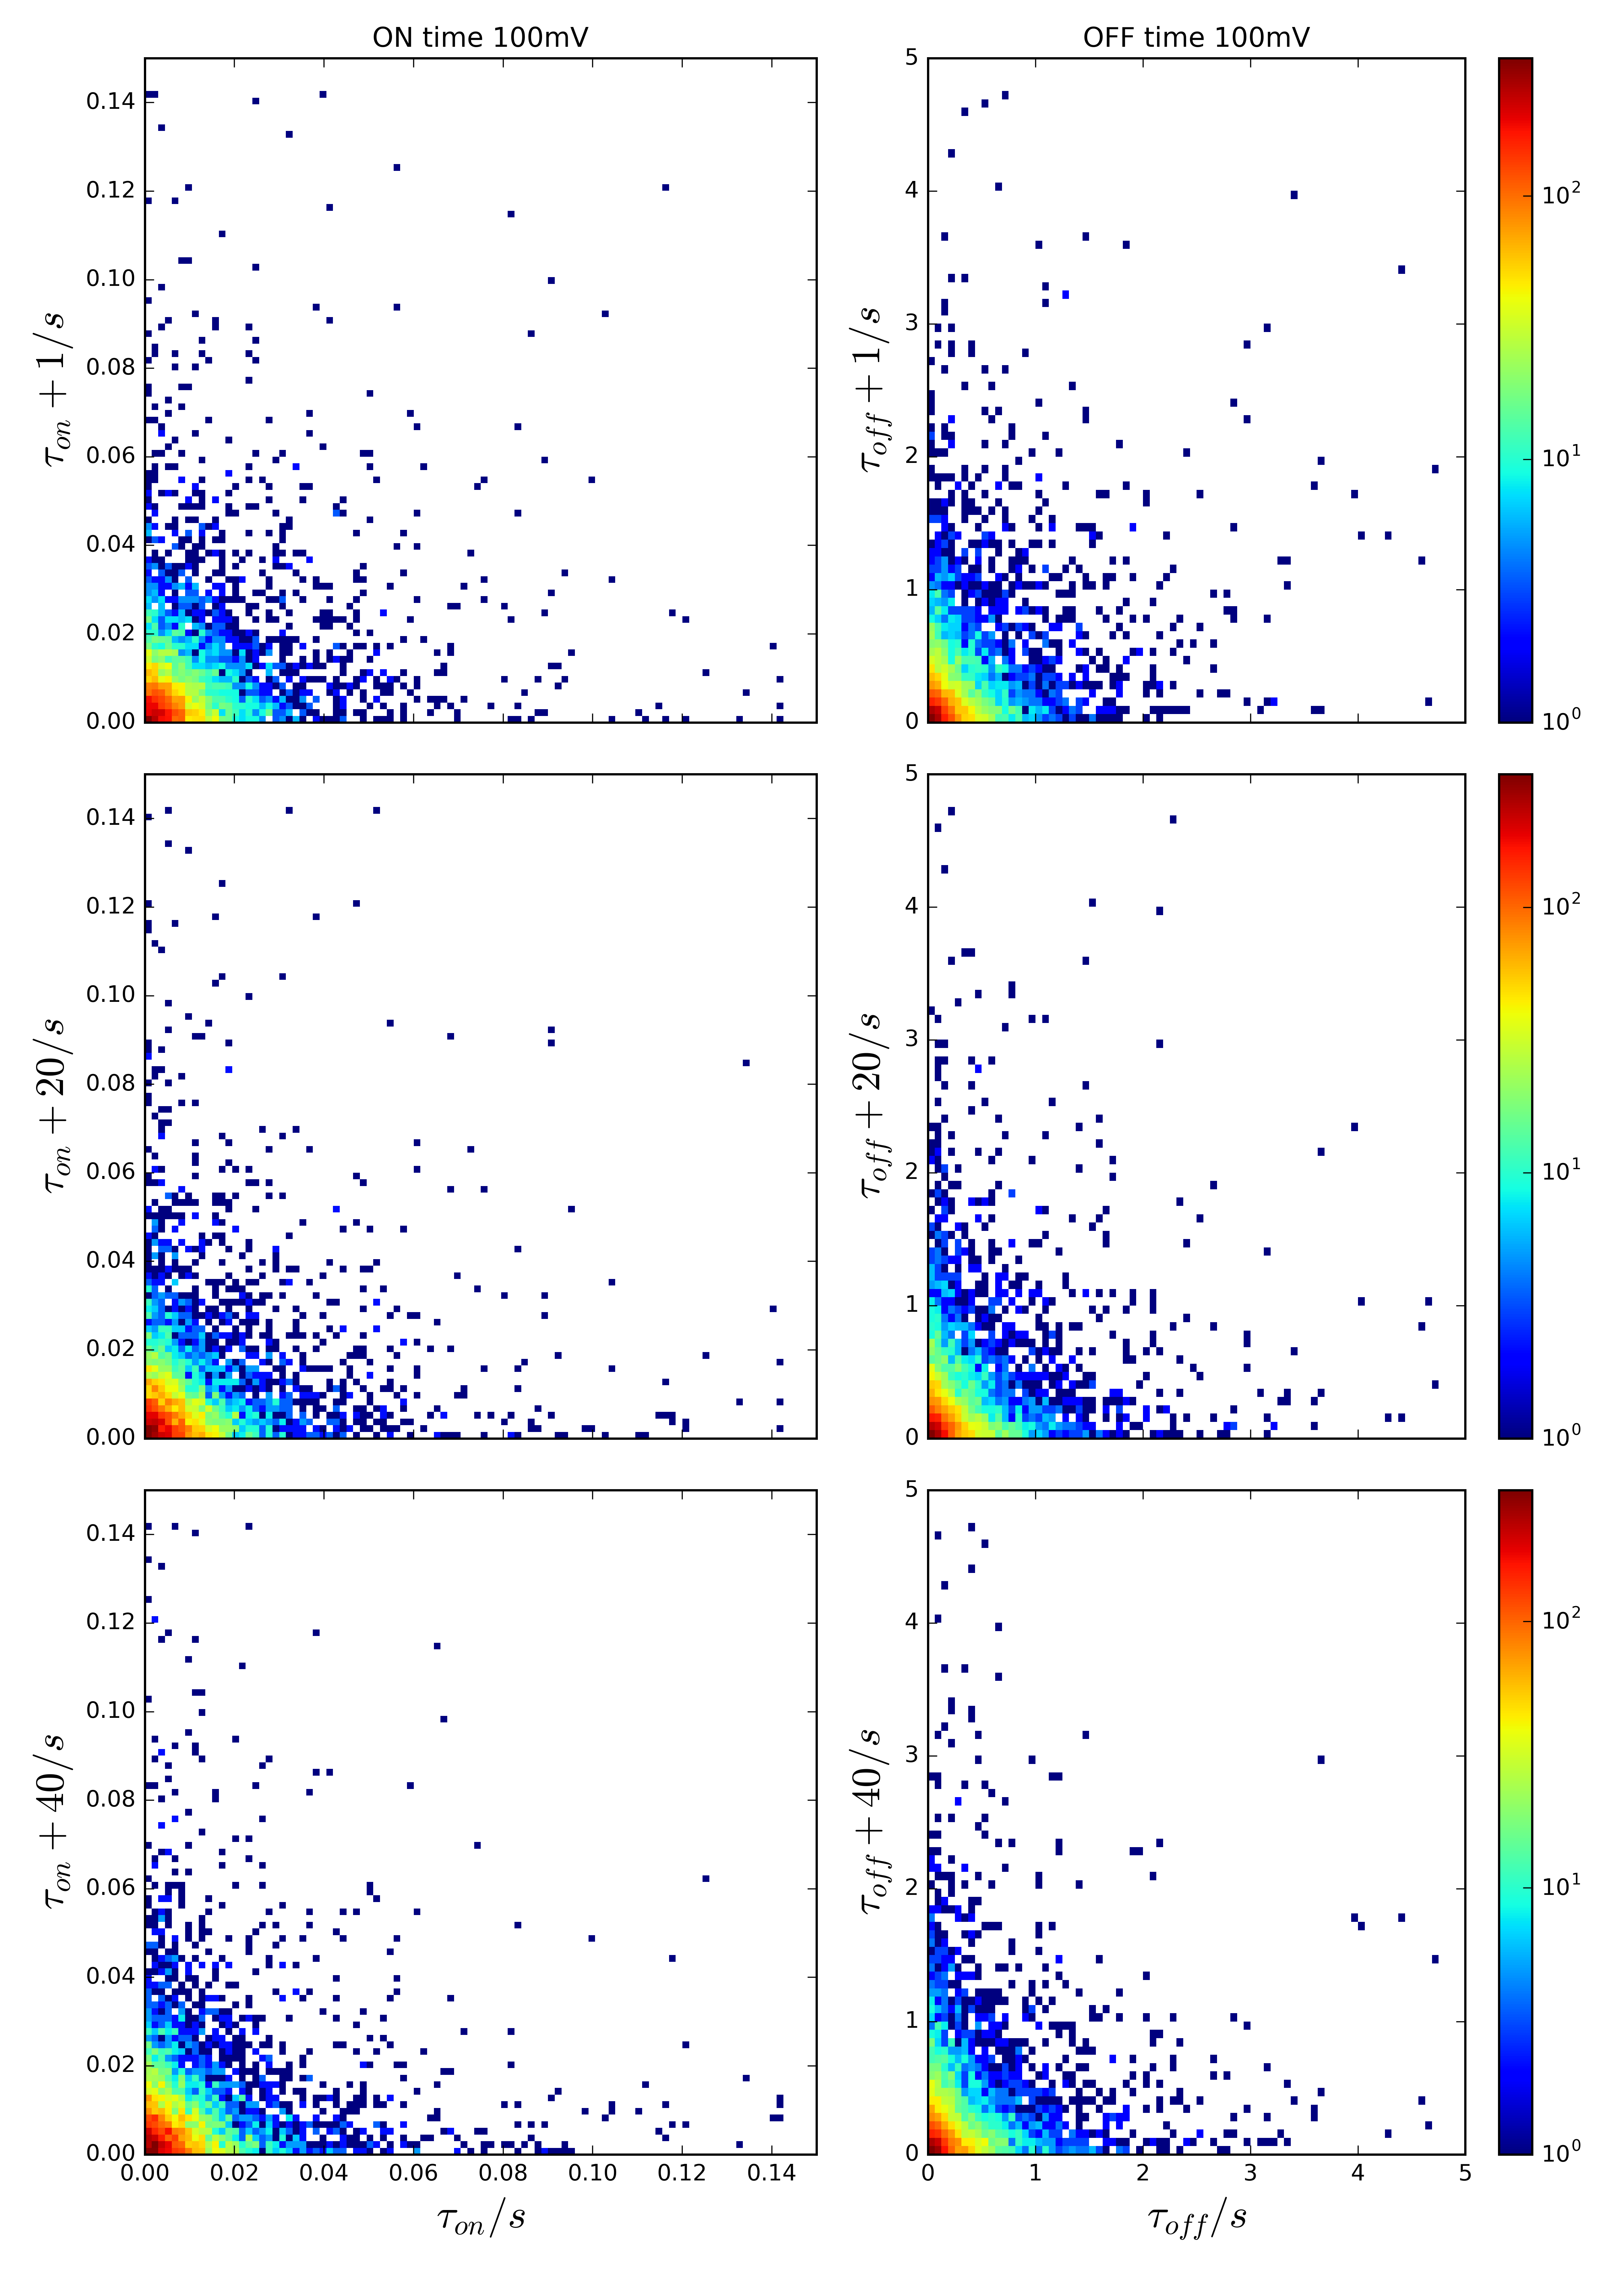
\includegraphics[width=.9\textwidth]{tauOnplots}
\caption{Correlation between the on- and off-times and the on- and off-times after a certain amount of turnovers for 31 single CuAz molecules at 100 mV potential. A strong memory is present even after 40 turnovers.}
\label{on_plotjes}
\end{figure}

\newpage

\begin{figure}[ht!]
\centering
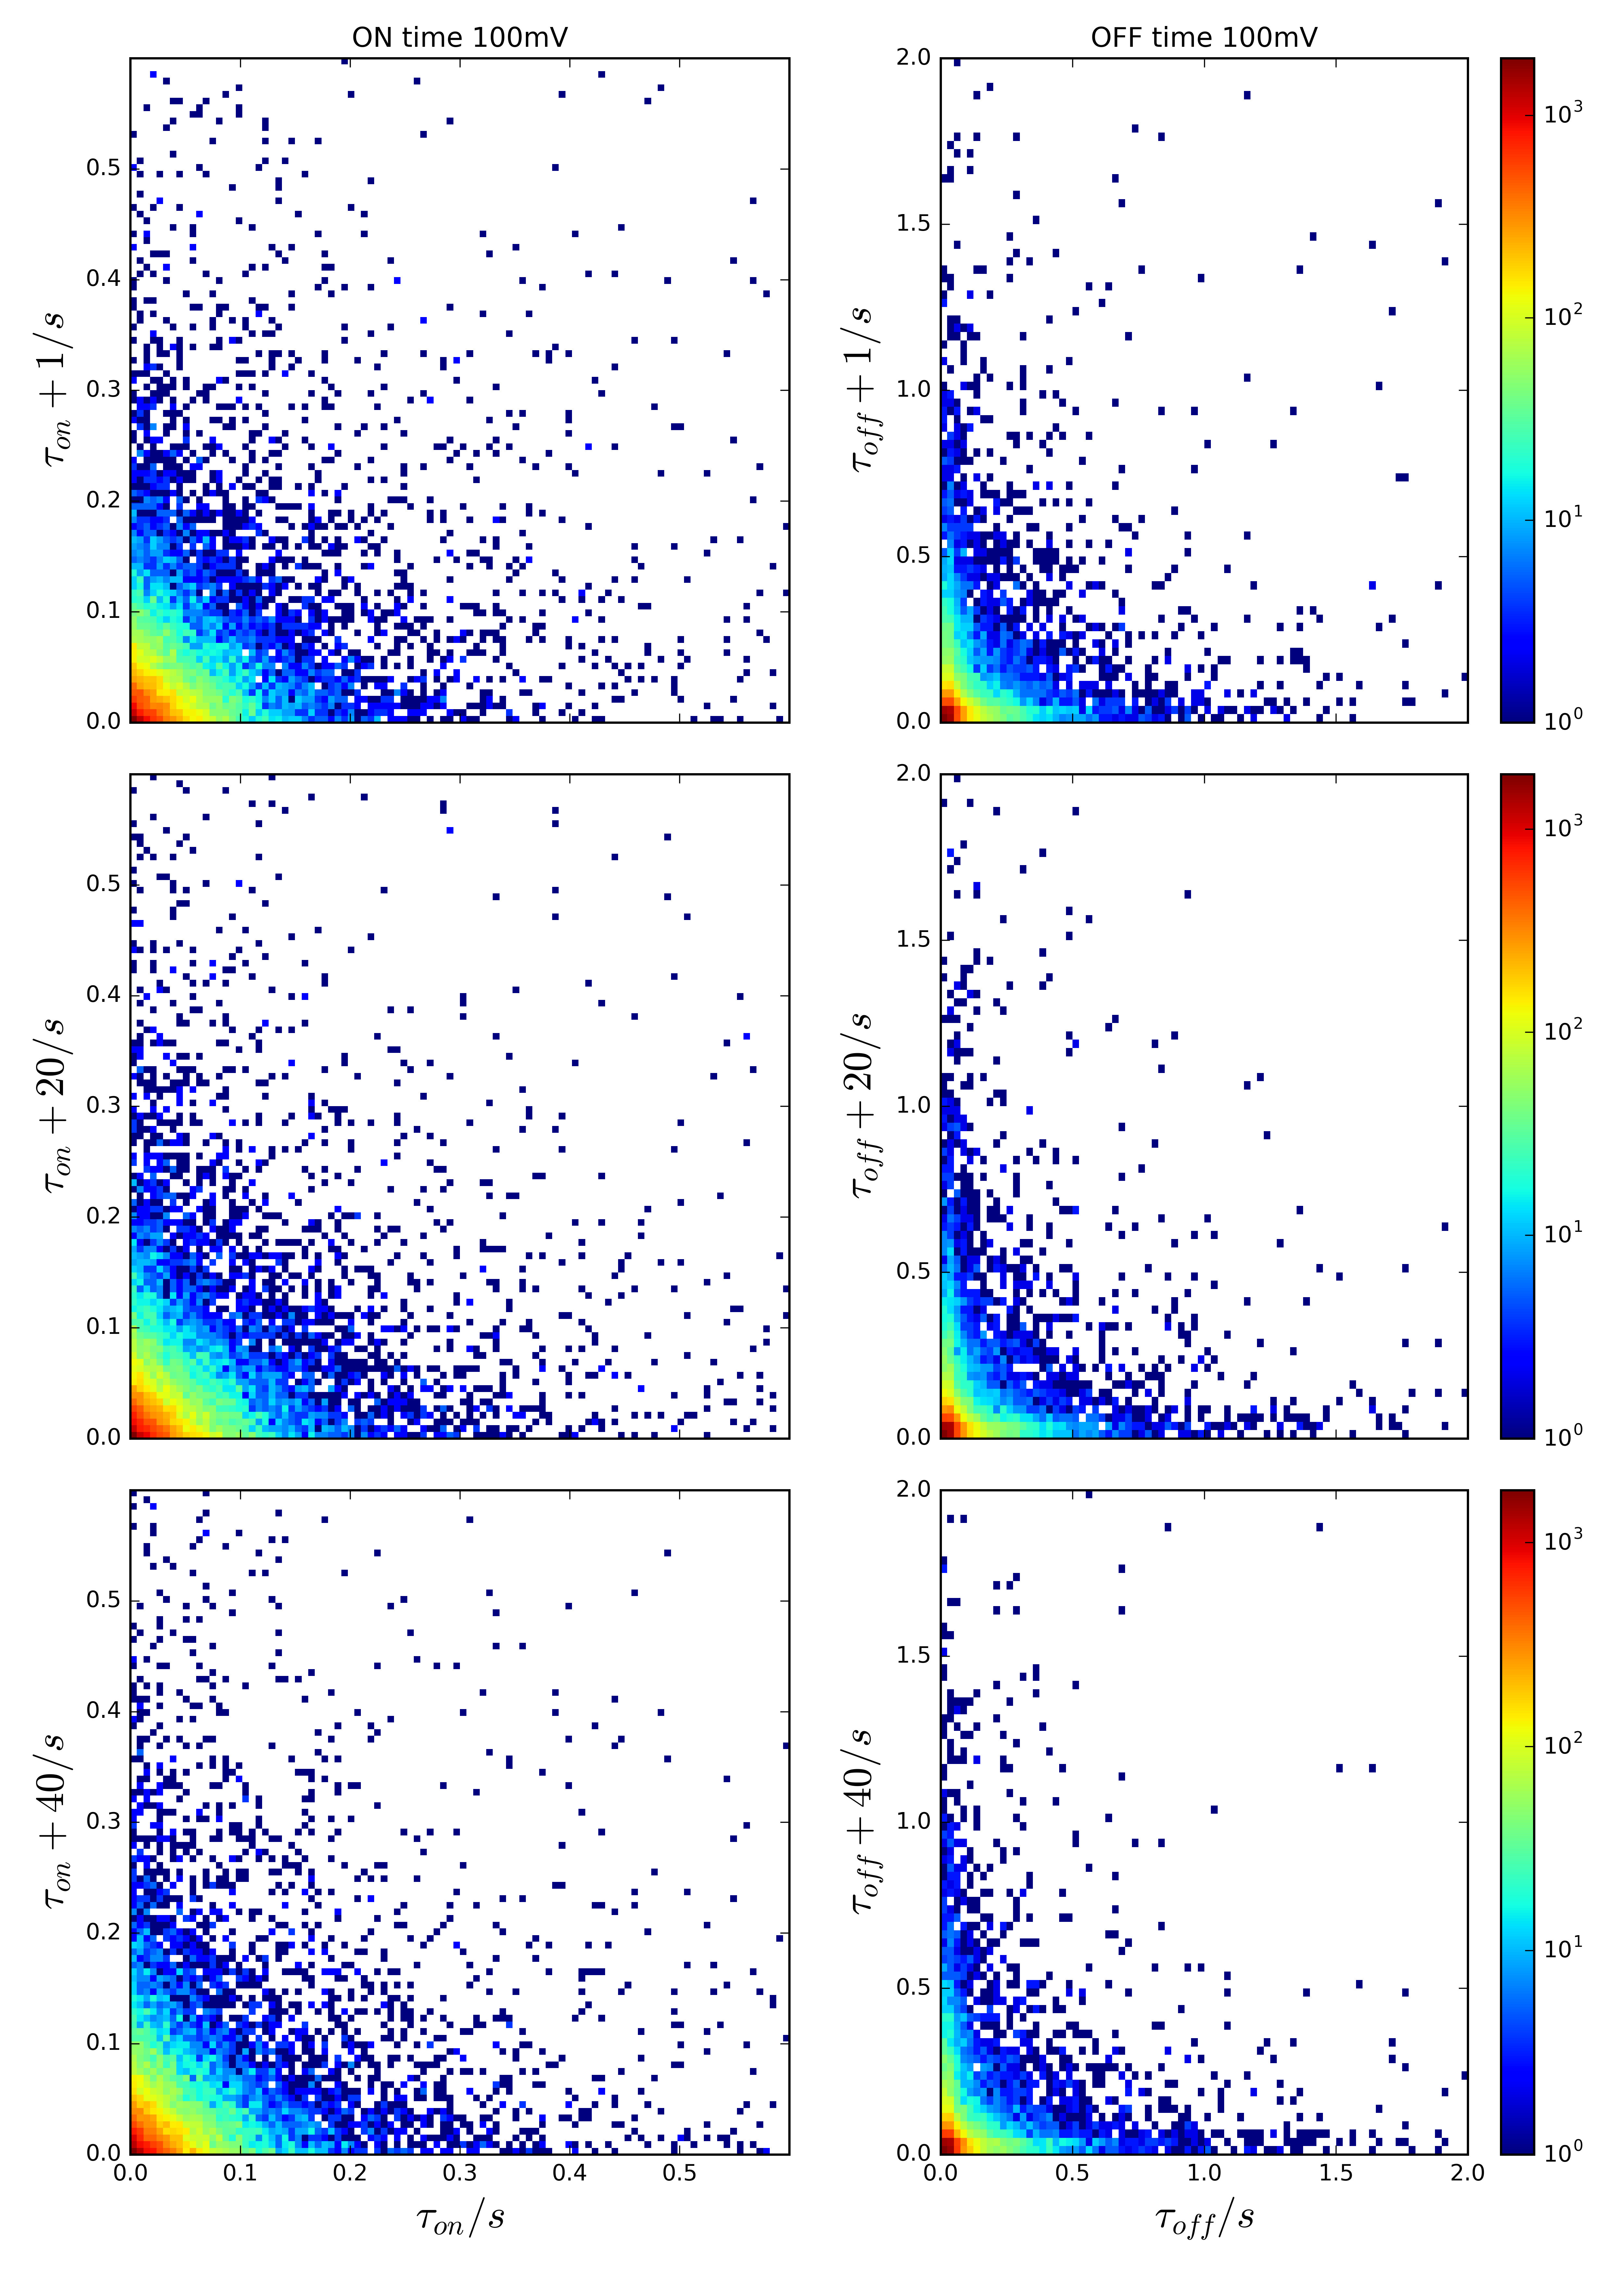
\includegraphics[width=.9\textwidth]{100mv_plus100}
\caption{Correlation between the on- and off-times and the on- and off-times after a certain amount of turnovers for 31 single CuAz molecules at 0 mV potential. Absence of memory after 1 turnover is visible for the off-times, where the on-times show memory.}
\label{on_plotjes_2}
\end{figure}

\newpage


An analogue way to describe the activity of turnover events separated by periods of low activity is with the Michaelis-Menten equation. According to the Michaelis-Menten mechanism, a substrate $S$ binds reversibly with enzyme $E$ to form the complex $ES$:

\begin{equation}\label{MMmech}
E + S \overset{k_{1}}{\underset{k_{-1}}\rightleftarrows} ES \overset{k_{2}}\rightarrow E^{0} + P,  \qquad E^{0} \overset{k_{3}}\rightarrow E.
\end{equation}
Then $ES$ produces $P$ and $E$ is regenerated for the next catalytic cycle. It has been proven that the Michaelis-Menten equation holds for single molecules according to the single-molecule Michaelis-Menten equation \cite{English2006}:
\begin{equation}\label{MMmech1}
\frac{1}{\langle \tau \rangle} = \frac{k_{2}[S]}{[S]+K_{M}},
\end{equation}
 where $K_{M}$ is the Michaelis constant. This process is similar to the redox of CuAz and can be seen when comparing equation \ref{ox_pros} with equation \ref{MMmech}. Instead of enzyme $E$ that forms a complex $ES$, we have the CuAz which forms a complex with reductant $R$. The product $P$ is the reduced $\textup{Cu}^{+}$ and the oxidation to $\textup{Cu}^{2+}$ ensures the next redox cycle. Further research on this subject might reveal new insights on the characterization of the memory effects, but is not done in this thesis.

\subsection{Autocorrelation CuAz} \label{autocor}

\begin{figure}[ht!]
\centering
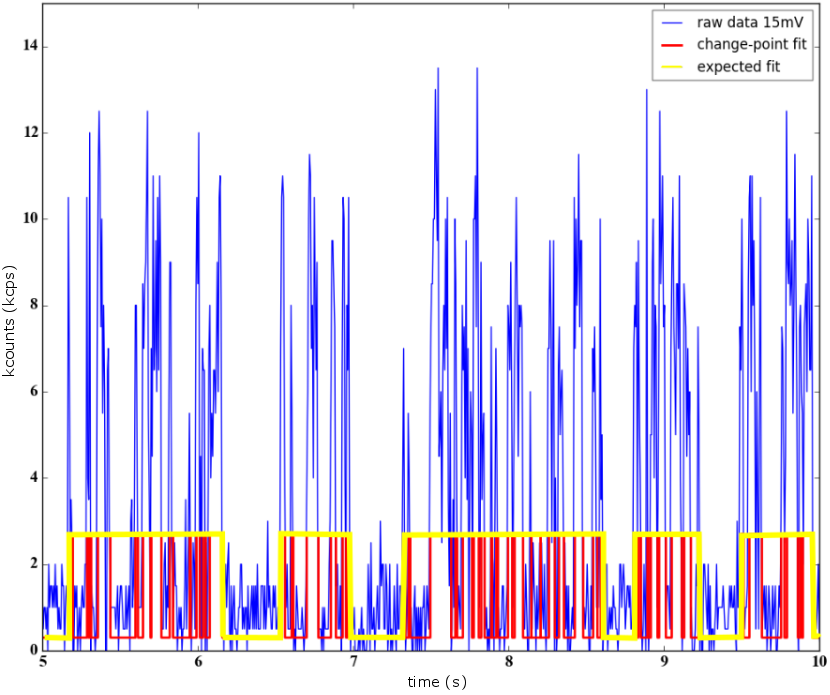
\includegraphics[width=\textwidth]{expected_fits}
\caption{A timetrace of CuAz at 15 mV potential as example of redox switching and blinking of the dye. The yellow line represents the switching due to the redox switching, while the red line shows the observed intensity jumps. Due to the blinking of the dye, the on-time of the CuAz is disturbed and instead of long on-times, the on-times are short.}
\label{expected_fit}
\end{figure}
When the solution is oxidized (at a potential of 40 mV or higher) the interaction between the dye and the solution is minimized. The intensity changes due to the blinking of the dye happen on a much bigger timescale than the redox switching and the on- and off-times calculated by the program are only due to the redox switching of the CuAz (i.e the blinking of the dye is not present in the timetraces for potentials higher than 40 mV). When the potential is changed to values below 40 mV the interaction between the dye and the solution becomes more prominent (shorter timescale) in the timetraces (the 25 mV and 0 mV timetraces in Figure \ref{plots_timetraces_diff_pot}). An example is shown in Figure \ref{expected_fit}. The long on-times, fitted with a yellow line, are due to the redox of the copper center. Due to the blinking of the dye, however, this long on-time is disturbed and divided into shorter on-times as is presented with the red line. In general it is hard to distinguish the on- and off-time due to blinking or switching below 40 mV by analyzing the timetraces.  A different way to distinguish which on- and off-time belong to the redox switching and which on- and off-time belong to the blinking of the dye is with the help of the autocorrelation. At higher potentials the autocorrelation can be fitted with a single exponential in the form of
\begin{equation} \label{single_exp}
g(\tau) =  A + Be^{-\tau/t_{1}}
\end{equation}
where $A$, $B$ and $t_{1}$ are constants. These constants are related to the on- and off-times via the equations
\begin{equation}\label{tau_on}
\frac{\tau_{off}}{\tau_{on}} = \frac{B}{A}
\end{equation}
and
\begin{equation}\label{tau_off}
\frac{1}{t_{1}} = \frac{1}{\tau_{on}} + \frac{1}{\tau_{off}}.
\end{equation}
These formulas have been used in similar autocorrelation analysis (\cite{Wai-TakYip1998},\cite{Vosch2007}). When the potential reaches values of 40 mV and below, the interaction between the dye and the reduced ascorbate and ferricyanide becomes prominent and the fit of the autocorrelation consists of two exponentials. In contradiction to what one would expect, this is NOT simply a sum of two exponentials, such as

\begin{equation}\label{multi_exp}
g(\tau) = A +  B_{1}e^{-\tau/t_{1}} + B_{2}e^{-\tau/t_{2}}. 
\end{equation}

The latter formula is valid if $t_{1}$ and $t_{2}$ are not correlated or if $t_{1} \gg t_{2}$ ($t_{1} \ll  t_{2}$). With $t_{1}$($t_{2}$) belonging to the redox switching and $t_{2}$($t_{1}$) to the blinking of the dye, this is clearly correlated. As mentioned before, for potentials below 40 mV the blinking of the dye becomes more prominent and the difference between $t_{1}$ and $t_{2}$ is within a few orders of magnitude. The mentioned sum of exponentials is for this case more complicated and up to this point in time the exact form of this exponent is not known. To keep things simple, only the (single exponential) autocorrelation for potentials higher than 40 mV, as described by equation \ref{single_exp}, will be used in this analysis.  




\subsection{Distribution midpoint potential CuAz}
To give the redox switching of the CuAz a more quantitative meaning, the average $\tau_{on}$ ($\bar{\tau}_{on}$) and average $\tau_{off}$ ($\bar{\tau}_{off}$) can be related to the Nernst equation since the switching is due to the redox reaction of CuAz. Rewriting equation \ref{nernst} to 

\begin{equation}\label{nernst_tau}
E = E^{0}+\frac{k_{B}T}{ne}\textup{ln}\left ( \frac{\bar{\tau}_{off}}{\bar{\tau}_{on}} \right )
\end{equation}
the average on- and off-times can be related to the potential applied. Rewriting equation \ref{nernst_tau} leads to
\begin{equation}\label{fit_onoff}
\frac{\bar{\tau}_{off}}{\bar{\tau}_{on}} = \textup{exp}\left ( \frac{E_{0}-E}{0.059} \right ).
\end{equation}
A fit through the ratio of the $\frac{\bar{\tau}_{off}}{\bar{\tau}_{on}}$ and the applied potential $E$ will lead to the midpoint potential $E^{0}$ of the protein. To extract the midpoint potential, two different methods are combined. The first method is the direct calculation of the on- and off-times from the timetraces with the use of the changepoint program written by  Lucas P. Watkins and Haw Yang. The second method uses exclusively the autocorrelation to find the ratio of  $\frac{\bar{\tau}_{off}}{\bar{\tau}_{on}}$ for any given potential. As discussed, only the potentials between 40 mV and 100 mV are analyzed. Another requirement is the activity of the molecule. Only CuAz that is still active after at least four different potentials has been taken in consideration. Using 42 different CuAz molecules, the distribution of 42 molecules is plotted in Figure \ref{t_ratio_plot} together with their Gaussian fit. The distribution of midpoint potentials acquired directly from the timetraces has a mean of 0.59 mV and a full width at half maximum (FWHM) of 24.58 mV. When the distribution is acquired from the autocorrelation, the mean is 5.12 mV and the FWHM is 24.95 mV. Such distribution of the midpoint potentials of CuAz has been reported earlier \cite{Salverda2010} where the midpoint potential was found to vary by tens of millivolts across the electrode surface   . This kind of difference in midpoint potentials has been reported by other similar experiments \cite{Zhang2017} and explained due to strong irradiation. Single molecules show lower mid-point potential when excited at higher intensity. This aspect has to be confirmed by further research in this specific case however. 

\begin{figure}[ht!]
\centering
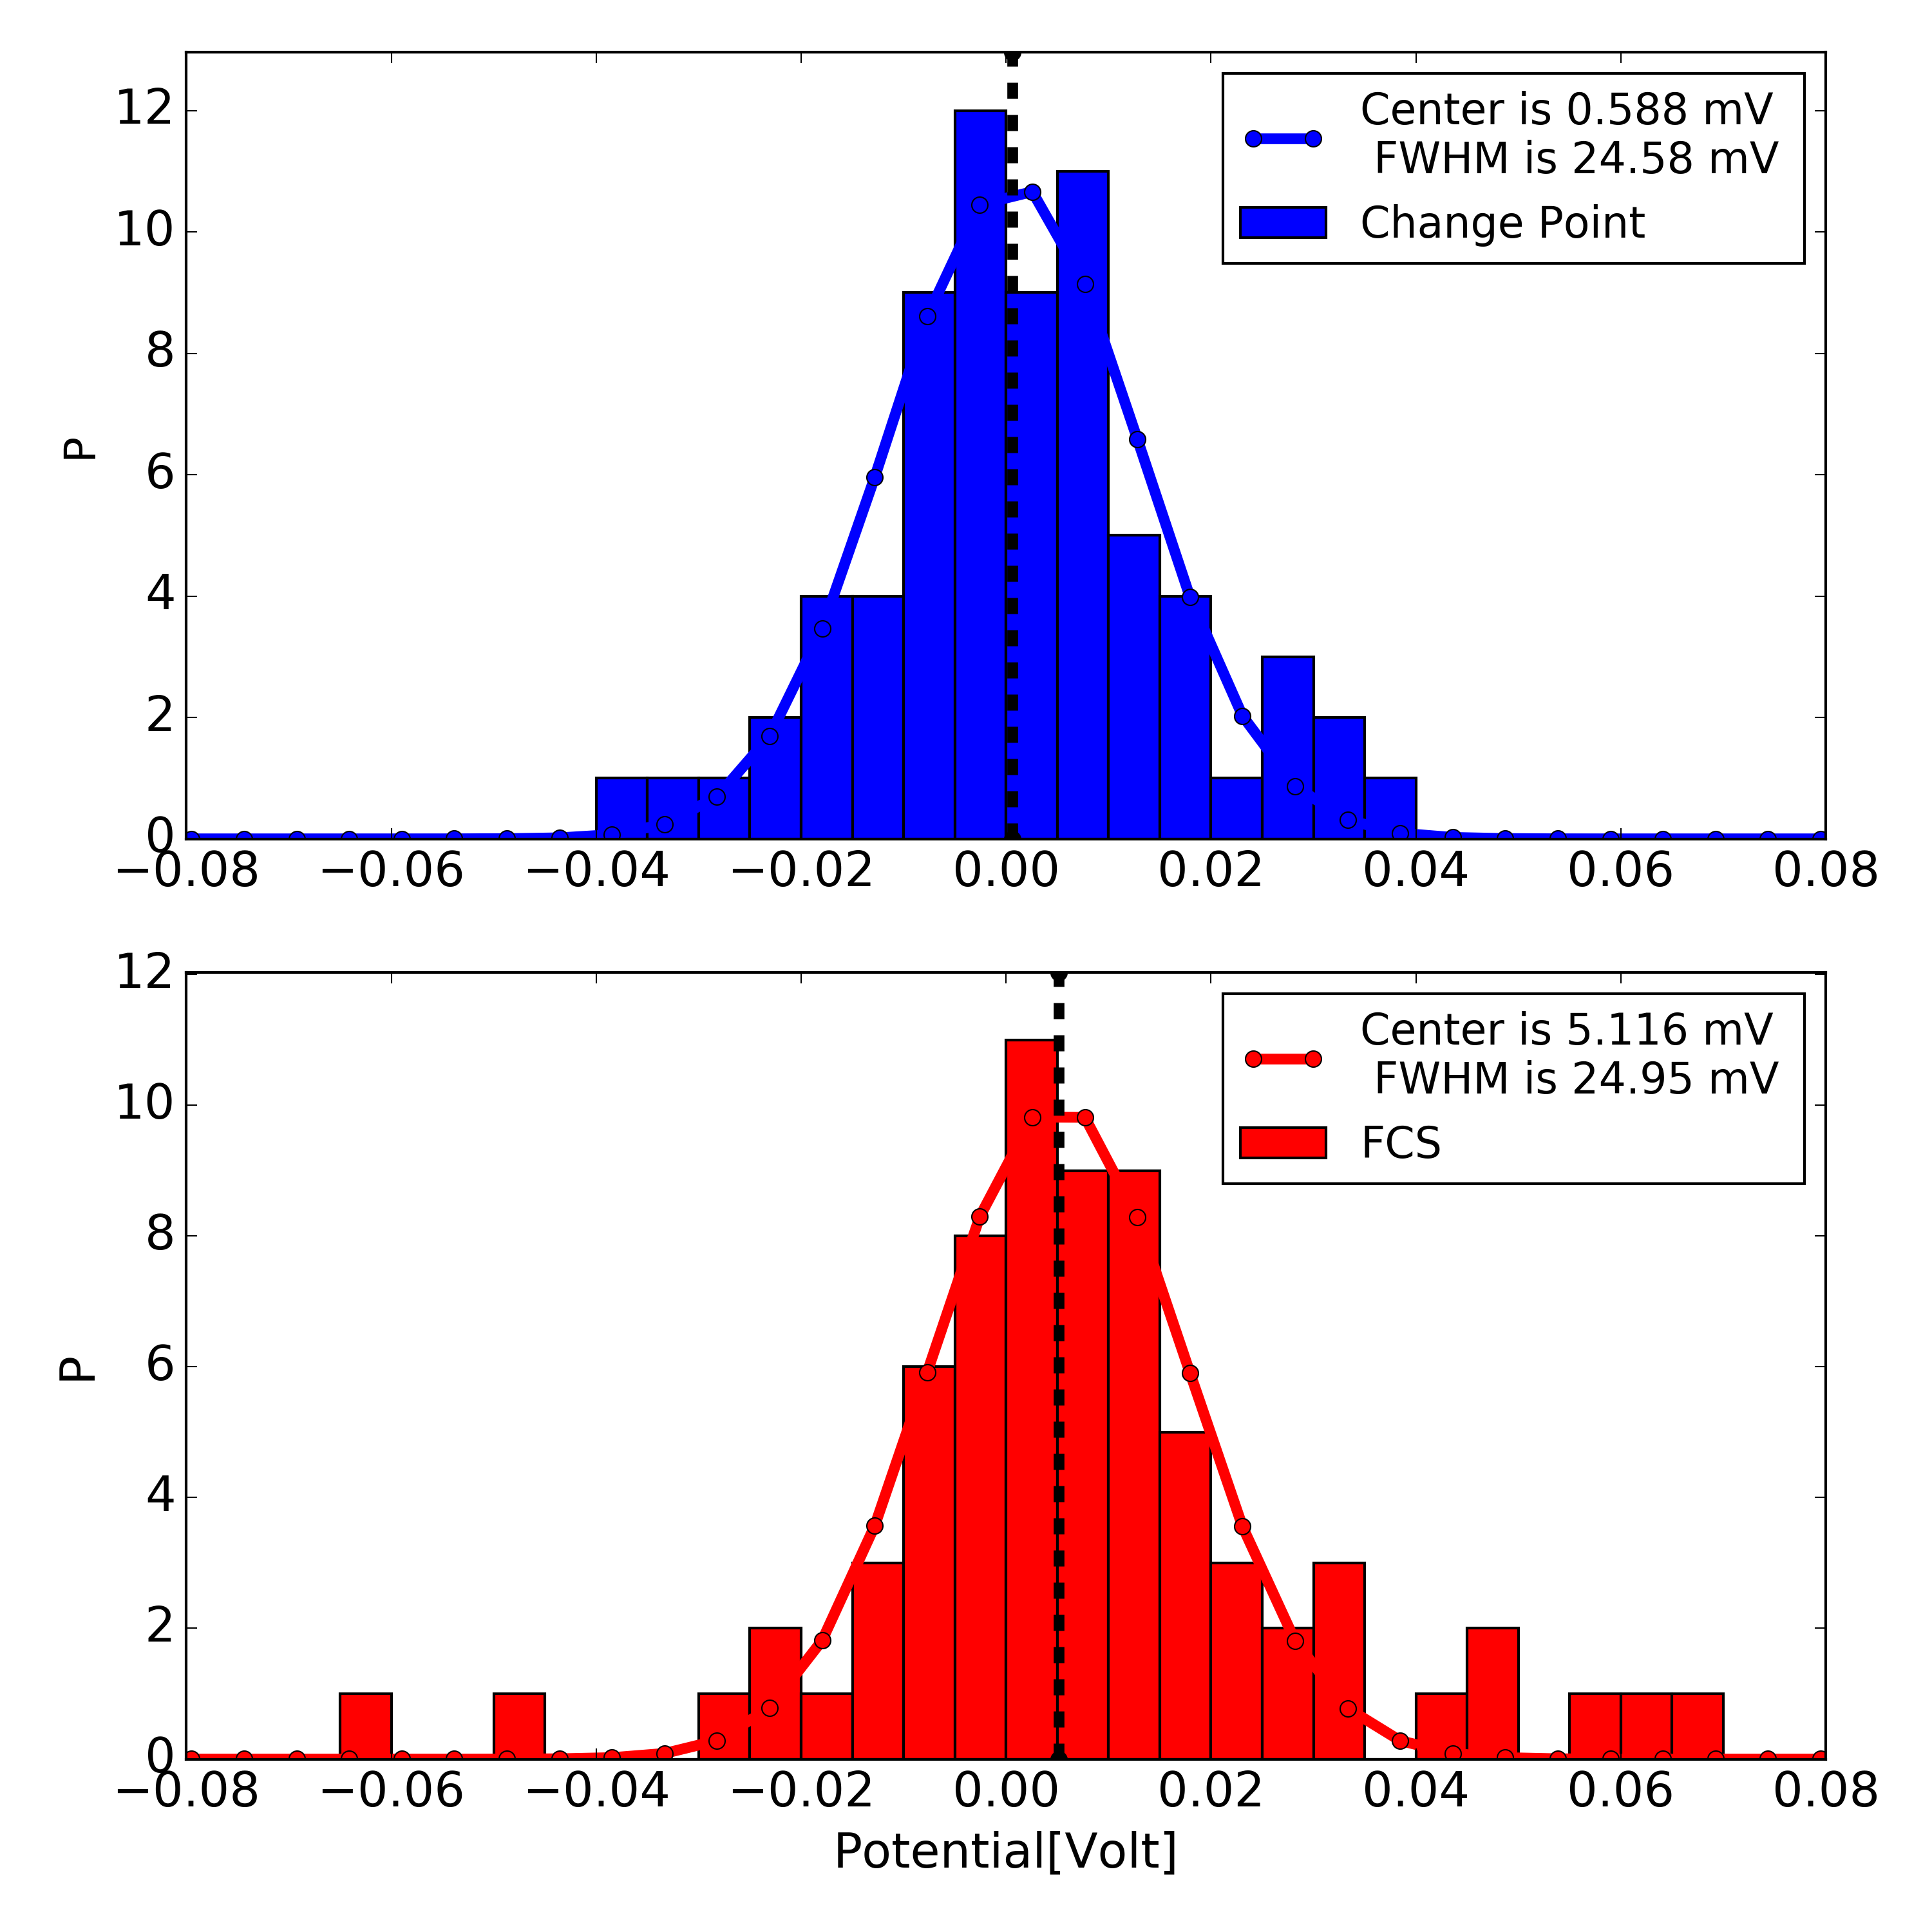
\includegraphics[width=\textwidth]{midpointhistograms}
\caption{Histogram and distribution of the midpoint potential of CuAz. Top: the distribution of the midpoint potential of CuAz acquired directly from the timetraces fitted with a Gaussian function. The mean is 0.59 mV and the FWHM is 24.58 mV. Bottom: the distribution acquired from the auto correlation. The mean is 5.12 mV and the FWHM is 24.95 mV.}
\label{t_ratio_plot}
\end{figure}

\bibliographystyle{lion-msc}
\bibliography{THESIS}

\end{document}
